% Курсовая работа, черновик 4 (27 октября 2026). Компилировать XeLaTeX:
%   latexmk -xelatex main.tex
% Оформление по ГОСТ 7.32-2017: поля 30/15/20/20 мм, 14 пт, полуторный интервал,
% абзацный отступ 1,25 см, заголовки структурных элементов прописными по центру.
\documentclass[a4paper,14pt]{extarticle}

\usepackage[no-math]{fontspec}
\setmainfont{Liberation Serif}  % метрически совпадает с Times New Roman; при наличии можно поставить Times New Roman
\setmonofont{Liberation Mono}[Scale=0.9]
\usepackage{polyglossia}
\setdefaultlanguage{russian}
\setotherlanguage{english}

\usepackage[left=30mm,right=15mm,top=20mm,bottom=20mm]{geometry}
\usepackage{setspace}
\onehalfspacing
\setlength{\parindent}{1.25cm}
\setlength{\emergencystretch}{3em}

\usepackage{amsmath,amssymb,amsthm}
\usepackage{graphicx}
\usepackage{float}
\usepackage{enumitem}
\setlist{nosep,leftmargin=*,labelindent=\parindent}
\usepackage{array}
\usepackage{caption}
\captionsetup[figure]{name=Рисунок,labelsep=endash,justification=centering,font={onehalfspacing}}
\captionsetup[table]{name=Таблица,labelsep=endash,justification=raggedright,singlelinecheck=false}
\usepackage{fancyvrb}
\usepackage{xurl}
\usepackage[hidelinks]{hyperref}

% Заголовки разделов: с абзацного отступа, полужирные, без точки; каждый раздел с новой страницы
\usepackage{titlesec}
\titleformat{\section}{\normalfont\bfseries}{\hspace*{\parindent}\thesection}{0.6em}{}
\titleformat{\subsection}{\normalfont\bfseries}{\hspace*{\parindent}\thesubsection}{0.6em}{}
\titlespacing*{\section}{0pt}{0pt}{12pt}
\titlespacing*{\subsection}{0pt}{12pt}{6pt}
\newcommand{\sectionbreak}{\clearpage}

% Заголовки структурных элементов: прописными по центру, в содержании без номера
\newcommand{\structsection}[1]{%
  \clearpage
  \phantomsection
  \addcontentsline{toc}{section}{#1}%
  \begin{center}\bfseries #1\end{center}\vspace{6pt}}

\usepackage{tocloft}
\renewcommand{\cfttoctitlefont}{\hfill\bfseries}
\renewcommand{\cftaftertoctitle}{\hfill}
\renewcommand{\cftsecfont}{\normalfont}
\renewcommand{\cftsecpagefont}{\normalfont}
\renewcommand{\cftsecleader}{\cftdotfill{\cftdotsep}}
\renewcommand{\contentsname}{СОДЕРЖАНИЕ}

\theoremstyle{plain}
\newtheorem{theorem}{Теорема}[section]
\newtheorem{lemma}[theorem]{Лемма}
\newtheorem{corollary}[theorem]{Следствие}
\newtheorem{proposition}[theorem]{Предложение}
\theoremstyle{definition}
\newtheorem{definition}[theorem]{Определение}
\newtheorem{task}{Задача}[section]
\theoremstyle{remark}
\newtheorem{remark}[theorem]{Замечание}
\renewcommand{\qedsymbol}{$\blacksquare$}

\newcommand{\sk}[2]{\langle #1,#2\rangle}
\newcommand{\R}{\mathbb{R}}
\newcommand{\Hb}{\mathbb{H}}
\DeclareMathOperator{\ch}{ch}
\DeclareMathOperator{\sh}{sh}
\DeclareMathOperator{\thh}{th}
\DeclareMathOperator{\arcth}{arth}
\newcommand{\todo}[1]{\textbf{[#1]}}

\begin{document}

% Титульный лист: входит в нумерацию, номер не ставится (ГОСТ 7.32-2017, 6.3.2)
\begin{titlepage}
\begin{singlespace}
\centering
Министерство просвещения Российской Федерации\\
федеральное государственное бюджетное образовательное учреждение\\
высшего образования\\
«Московский педагогический государственный университет»

\vspace{1.2cm}
Институт математики и информатики\\
Кафедра геометрии им.~Л.\,С.~Атанасяна

\vspace{2cm}
{\bfseries КУРСОВАЯ РАБОТА}

\vspace{0.8cm}
По дисциплине: ГЕОМЕТРИЯ\\[4pt]
На тему: {\bfseries ИНТЕРПРЕТАЦИЯ УТВЕРЖДЕНИЙ ГЕОМЕТРИИ ЛОБАЧЕВСКОГО В МОДЕЛИ КЭЛИ~--- КЛЕЙНА И ИХ КОМПЬЮТЕРНАЯ ВИЗУАЛИЗАЦИЯ}

\vspace{0.8cm}
Код и направление подготовки: 44.03.05 Педагогическое образование\\
(с двумя профилями подготовки)\\
Направленность (профиль) образовательной программы:\\
Математика и экономика

\vspace{1.2cm}
\begin{minipage}[t]{0.45\textwidth}
\raggedright
«Допуск к защите»\\[2pt]
\rule{5cm}{0.4pt}\\
{\small (к защите / снять с защиты)}

\vspace{1cm}
Проверка на объём заимствований:\\
\rule{2cm}{0.4pt}\,\% авторского текста
\end{minipage}\hfill
\begin{minipage}[t]{0.5\textwidth}
\raggedleft
Выполнила:\\
студентка 3 курса, группа № 305\\
Булгакова Мария Владимировна

\vspace{0.6cm}
Научный руководитель:\\
\todo{должность, учёная степень}\\
\todo{ФИО руководителя}

\vspace{0.6cm}
«Оценка» \rule{2.5cm}{0.4pt}\\
{\small (итоговая сумма баллов / оценка)}
\end{minipage}

\vfill
Москва~--- 2026
\end{singlespace}
\end{titlepage}
\setcounter{page}{2}


\begin{center}\bfseries СОДЕРЖАНИЕ\end{center}
\makeatletter\@starttoc{toc}\makeatother

\structsection{ВВЕДЕНИЕ}

Утверждение «через точку вне прямой проходят по крайней мере две прямые, не пересекающие её» нельзя проверить на листе бумаги. Чертёж подчиняется евклидовой геометрии, и любая попытка нарисовать две непересекающиеся прямые через одну точку заканчивается тем, что они где-нибудь сходятся. Поэтому геометрию Лобачевского строят аксиоматически, а каждое доказательство опирается только на аксиомы и уже доказанные теоремы.

Модель Кэли~--- Клейна позволяет посмотреть на ту же геометрию с другой стороны. Точками в ней служат точки круга, прямыми~--- хорды, и все аксиомы абсолютной геометрии вместе с аксиомой Лобачевского в ней выполняются. Значит, каждая теорема геометрии Лобачевского верна и в модели, и её можно увидеть на конкретной фигуре. Обратное неверно: рисунок в модели ничего не доказывает, он лишь показывает один из случаев. В этой работе модель используется в обоих качествах. Как интерпретация она показывает, что означает утверждение. Как вычислительный инструмент она даёт явные формулы для угла параллельности, расстояния до прямой, углов четырёхугольника Саккери.

Компьютерная модель добавляет к этому движение. Если точку на рисунке можно передвинуть, становится видно, какие величины меняются вместе с ней, а какие остаются постоянными, и в какой момент пересекающиеся прямые становятся параллельными, а затем расходящимися. Чтобы числа на экране совпадали с теоремами, все построения в работе выведены из формул модели и проверены численно.

\textbf{Объект исследования}: планиметрия и простейшие объекты стереометрии Лобачевского.

\textbf{Предмет исследования}: интерпретация утверждений геометрии Лобачевского в модели Кэли~--- Клейна и их компьютерная визуализация.

\textbf{Цель работы}: построить в модели Кэли~--- Клейна интерпретации основных утверждений планиметрии Лобачевского, вывести для них явные формулы и создать по этим формулам интерактивные компьютерные модели.

Задачи работы:
\begin{enumerate}
  \item описать модель Кэли~--- Клейна на языке абсолюта: полюс и поляра, сложное отношение, π-движения, симметрия относительно прямой;
  \item интерпретировать в модели параллельные и расходящиеся прямые, угол параллельности, общий перпендикуляр и вывести формулу Лобачевского для угла параллельности;
  \item интерпретировать утверждения о треугольниках и четырёхугольниках, которые являются отрицаниями утверждений, равносильных V постулату;
  \item показать, как модель доказывает непротиворечивость геометрии Лобачевского относительно евклидовой и независимость аксиомы параллельности;
  \item распространить построение на пучки прямых, связки прямых и простейшие поверхности пространства Лобачевского;
  \item создать интерактивную веб-страницу с моделями плоскости и пространства Лобачевского;
  \item составить и решить задачи по теме работы.
\end{enumerate}

\textbf{Методы исследования}: аксиоматический метод, метод моделей, аналитический метод в однородных координатах, численная проверка формул.

Собственные результаты автора: вывод формул разделов 2 и~3 в модели Кэли~--- Клейна (угол параллельности с вершиной в центре круга, расстояние от точек прямой до другой прямой, углы четырёхугольника Саккери, граничная точка в отрицании предложения Лежандра); теорема о траекториях пучков и связок (теоремы~\ref{thm:traektoriya} и~\ref{thm:svyazka}) с доказательством, в котором три случая разбираются одним рассуждением; построение комнаты с полом-орисферой (теорема~\ref{thm:komnata}); веб-страница «Круг Кэли~--- Клейна» с моделями плоскости и пространства; решения задач раздела~7. Определения и классические теоремы приводятся по учебникам Л.\,С.~Атанасяна~[1], Л.\,С.~Атанасяна и В.\,Т.~Базылева~[2], Н.\,В.~Ефимова~[3].

Работа состоит из введения, семи разделов, заключения, списка использованных источников и приложения. Разделы~1--4 посвящены плоскости Лобачевского. Разделы~5 и~6 переносят те же методы на пространство: пучки и связки прямых, сферу, орисферу и эквидистантную поверхность, многогранники-«комнаты». Раздел~7 содержит задачи с решениями.

\section{Модель Кэли~--- Клейна плоскости Лобачевского}

\subsection{Аксиома Лобачевского}

Абсолютной геометрией называют систему аксиом Гильберта без аксиомы параллельности: аксиомы принадлежности (I), порядка (II), конгруэнтности (III) и непрерывности (IV)~[2]. Её теоремы верны и в геометрии Евклида, и в геометрии Лобачевского. Геометрия Лобачевского получается, если к аксиомам I--IV добавить отрицание аксиомы параллельности Евклида.

\begin{definition}[аксиома Лобачевского]
На плоскости существуют прямая $a_0$ и не лежащая на ней точка $A_0$, такие, что через $A_0$ проходят по крайней мере две прямые, не пересекающие $a_0$~[1,~2].
\end{definition}

\begin{theorem}[\!\!{[1]}]\label{thm:lv-vsegda}
Для любой прямой $a$ и любой не лежащей на ней точки $A$ через $A$ проходят по крайней мере две прямые, не пересекающие $a$.
\end{theorem}
\begin{proof}
Допустим, что через $A$ проходит единственная прямая $h$, не пересекающая $a$. Опустим перпендикуляр $AB$ на $a$; перпендикуляр к $AB$ в точке $A$ не пересекает $a$, поэтому совпадает с $h$. Возьмём на $a$ произвольную точку $C$ и отложим от луча $AC$ в полуплоскости, не содержащей $B$, угол $CAM$, равный углу $ACB$. Прямая $AM$ не пересекает $a$ (иначе внешний угол треугольника был бы равен внутреннему, не смежному с ним), поэтому $AM=h$. Тогда сумма углов прямоугольного треугольника $ABC$ равна $\angle B+\angle C+(\angle BAM-\angle CAM)=\pi/2+\angle C+\pi/2-\angle C=\pi$. По второй теореме Лежандра (теорема~\ref{thm:lezhandr2}) отсюда следует аксиома Евклида, что противоречит аксиоме Лобачевского.
\end{proof}

Если $h_1$ и $h_2$~--- две прямые, проходящие через $A$ и не пересекающие $a$, то любая прямая через $A$, лежащая внутри одного из вертикальных углов, образованных $h_1$ и $h_2$ и не содержащих $a$, тоже не пересекает $a$. Поэтому таких прямых бесконечно много.

\subsection{Модель}

Зафиксируем на евклидовой плоскости единичную окружность $\omega$ с центром $O$ и будем называть её \emph{абсолютом}. Следуя~[1,~3], назовём \emph{π-точками} внутренние точки круга, \emph{π-прямыми}~--- хорды без концов, а отношение «π-точка $B$ лежит между $A$ и $C$» определим как то же отношение на евклидовом отрезке. Отношение принадлежности и отношение «между» совпадают с евклидовыми, поэтому аксиомы групп I и II в модели выполнены. Аксиомы непрерывности выполнены потому, что они выполнены на евклидовых отрезках~[1].

Для дальнейшего удобно записывать точки однородными координатами $X=(x_0:x_1:x_2)$, где точке $k=(k_1,k_2)$ плоскости отвечает $X=(1:k_1:k_2)$. Уравнение абсолюта принимает вид $-x_0^2+x_1^2+x_2^2=0$. Его левой части соответствует симметричная билинейная форма
\begin{equation}\label{eq:forma}
\sk{X}{Y}=-x_0y_0+x_1y_1+x_2y_2,
\end{equation}
которую мы будем называть \emph{формой абсолюта}. Точка $X$ лежит внутри круга, если $\sk{X}{X}<0$, на абсолюте, если $\sk{X}{X}=0$, и вне круга, если $\sk{X}{X}>0$.

\begin{definition}
\emph{Полярой} точки $P$ относительно абсолюта называется прямая $\{X:\ \sk{X}{P}=0\}$, а $P$~--- \emph{полюсом} этой прямой.
\end{definition}

Прямая $a_0+a_1k_1+a_2k_2=0$ имеет полюс $P=(-a_0:a_1:a_2)$. Из курса проективной геометрии~[3,~7] известно: поляра внешней точки~--- прямая, проходящая через точки касания двух касательных, проведённых из этой точки к абсолюту; поляра точки абсолюта~--- касательная в этой точке; поляра внутренней точки не пересекает круг. Следовательно, каждая π-прямая имеет полюс вне круга (или в бесконечно удалённой точке, если хорда~--- диаметр): это точка пересечения касательных к абсолюту в концах хорды. Отношение «полюс~--- поляра» взаимно: точка $X$ лежит на поляре точки $P$ тогда и только тогда, когда $P$ лежит на поляре $X$.

\subsection{π-движения и расстояние}

\begin{definition}[\!\!{[1]}]
\emph{π-движением} называется взаимно однозначное отображение круга на себя, которое переводит хорды в хорды и сохраняет сложное отношение любых четырёх точек одной прямой. π-фигуры называются \emph{равными}, если одна переводится в другую π-движением.
\end{definition}

Отображения круга на себя, переводящие хорды в хорды, являются проективными преобразованиями, сохраняющими абсолют. В однородных координатах они задаются матрицами $M$, для которых $\sk{MX}{MY}=\sk{X}{Y}$~[3]. Примеры: поворот вокруг $O$, симметрия относительно диаметра и \emph{сдвиг вдоль диаметра}
\begin{equation}\label{eq:sdvig}
M_t=\begin{pmatrix}\ch t&\sh t&0\\ \sh t&\ch t&0\\ 0&0&1\end{pmatrix},
\end{equation}
который переводит центр $O=(1:0:0)$ в точку $(\ch t:\sh t:0)$, то есть в точку $(\thh t,\,0)$ круга. Сохранение формы проверяется перемножением: $-(\ch t\,x_0+\sh t\,x_1)^2+(\sh t\,x_0+\ch t\,x_1)^2=-x_0^2+x_1^2$. Комбинируя сдвиги и повороты, можно перевести любую π-точку в центр круга. Проверка аксиом III группы для так определённого равенства фигур проведена в~[1].

\begin{definition}
Длиной отрезка $AB$ в модели называется число
\begin{equation}\label{eq:dlina}
d(A,B)=\tfrac12\bigl|\ln(AB,UV)\bigr|,
\end{equation}
где $U$, $V$~--- концы хорды $AB$, а $(AB,UV)$~--- сложное отношение четырёх точек.
\end{definition}

π-движения сохраняют сложное отношение и переводят концы хорды в концы хорды, поэтому равные отрезки имеют равные длины. Для вычислений удобнее другая запись той же величины.

\begin{proposition}\label{prop:ch}
Если $A$ и $B$~--- π-точки, а $A$, $B$ обозначают также их однородные координаты, то
\begin{equation}\label{eq:ch}
\ch d(A,B)=\frac{|\sk{A}{B}|}{\sqrt{\sk{A}{A}\,\sk{B}{B}}}.
\end{equation}
В координатах круга, при $A=(1:a)$, $B=(1:b)$, это равенство принимает вид $\ch d=\dfrac{1-a\cdot b}{\sqrt{(1-|a|^2)(1-|b|^2)}}$.
\end{proposition}
\begin{proof}
Точки прямой $AB$ имеют однородные координаты $A+tB$, и параметр $t$~--- проективный параметр на этой прямой: точке $A$ отвечает $t=0$, точке $B$ отвечает $t=\infty$. Сложное отношение четырёх точек равно сложному отношению их параметров, поэтому для концов хорды с параметрами $t_1$, $t_2$
\[
(AB,UV)=\frac{t_1-0}{t_1-\infty}:\frac{t_2-0}{t_2-\infty}=\frac{t_1}{t_2}.
\]
Концы хорды лежат на абсолюте, то есть $t_1$, $t_2$~--- корни уравнения $\sk{A}{A}+2t\sk{A}{B}+t^2\sk{B}{B}=0$. Обозначим $\alpha=\sk{A}{A}<0$, $\gamma=\sk{B}{B}<0$, $\beta=\sk{A}{B}$ и $\lambda=|\beta|/\sqrt{\alpha\gamma}$. Неравенство $\lambda\ge1$ следует из того, что уравнение имеет действительные корни. Корни равны $t_{1,2}=\bigl(-\beta\pm\sqrt{\beta^2-\alpha\gamma}\bigr)/\gamma$, их произведение $\alpha/\gamma$ положительно, и
\[
\frac{t_1}{t_2}=\Bigl(\frac{\lambda+\sqrt{\lambda^2-1}}{\lambda-\sqrt{\lambda^2-1}}\Bigr)^{\pm1}=\bigl(\lambda+\sqrt{\lambda^2-1}\bigr)^{\pm2}=e^{\pm2\operatorname{arch}\lambda}.
\]
Отсюда $\tfrac12|\ln(AB,UV)|=\operatorname{arch}\lambda$, что и требовалось. Вторая формула получается подстановкой $A=(1,a)$, $B=(1,b)$ в~\eqref{eq:forma}.
\end{proof}

\begin{corollary}\label{cor:ot-centra}
Расстояние от центра круга до π-точки $k$ равно $\operatorname{arth}|k|$. В частности, точка, удалённая от центра на расстояние $x$, изображается точкой на расстоянии $\thh x$ от $O$.
\end{corollary}

Из следствия видно, почему равные отрезки на рисунке модели выглядят по-разному. Отрезки длины $0{,}5$, отложенные подряд от точки $A$, на рисунке сжимаются к краю круга, и бесконечно много таких отрезков помещается на каждой хорде (рисунок~\ref{fig:lineyka}). В интерактивной модели (приложение~А) это видно в сценах «Модель Кэли~--- Клейна» и «π-движения»: при переносе треугольника к абсолюту длины его сторон и углы на панели остаются прежними, а сам треугольник на рисунке уменьшается.

\begin{figure}[H]
\centering
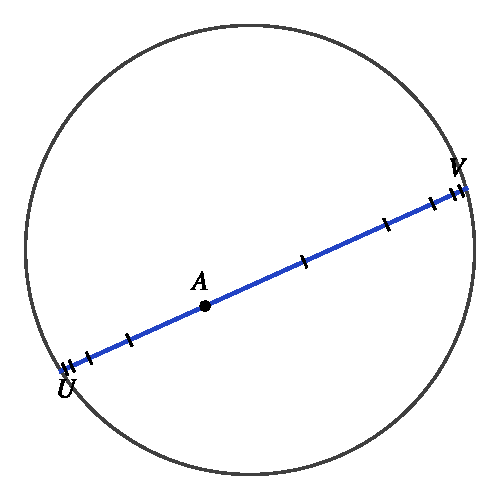
\includegraphics[width=0.46\textwidth]{fig/lineyka.pdf}
\caption{Отрезки длины $0{,}5$, отложенные от точки $A$ в обе стороны по хорде $UV$}
\label{fig:lineyka}
\end{figure}

\subsection{Симметрия относительно прямой и перпендикулярность}

\begin{proposition}\label{prop:simmetriya}
Пусть $\ell$~--- π-прямая, $P$~--- её полюс. Отображение
\begin{equation}\label{eq:otrazhenie}
\sigma_\ell(X)=X-2\,\frac{\sk{X}{P}}{\sk{P}{P}}\,P
\end{equation}
является π-движением, оставляет на месте каждую точку прямой $\ell$, отлично от тождественного и удовлетворяет условию $\sigma_\ell\circ\sigma_\ell=\mathrm{id}$. Это симметрия относительно прямой $\ell$.
\end{proposition}
\begin{proof}
Отображение линейно. Раскрывая скобки, получаем
\[
\sk{\sigma_\ell X}{\sigma_\ell Y}=\sk{X}{Y}-4\frac{\sk{X}{P}\sk{Y}{P}}{\sk{P}{P}}+4\frac{\sk{X}{P}\sk{Y}{P}\sk{P}{P}}{\sk{P}{P}^2}=\sk{X}{Y},
\]
то есть форма абсолюта сохраняется, и $\sigma_\ell$~--- π-движение. Точки прямой $\ell$ удовлетворяют условию $\sk{X}{P}=0$ и остаются на месте. Наконец, $\sigma_\ell(P)=-P$ (та же точка в однородных координатах), и $\sigma_\ell(\sigma_\ell X)=X$ проверяется подстановкой.
\end{proof}

Формула~\eqref{eq:otrazhenie} показывает, что $\sigma_\ell(X)$ лежит на прямой $XP$. Это даёт простое описание перпендикулярности в модели, которое приводится в курсе как построение: перпендикуляр к хорде проводится через её полюс.

\begin{lemma}\label{lem:polyus}
Пусть $m$ и $\ell$~--- π-прямые. Прямая $m$ перпендикулярна $\ell$ тогда и только тогда, когда прямая, содержащая хорду $m$, проходит через полюс $P$ прямой $\ell$.
\end{lemma}
\begin{proof}
Пусть $m$ пересекает $\ell$ в точке $C$. Прямая $m$ перпендикулярна $\ell$ тогда и только тогда, когда она совпадает со своим образом при симметрии $\sigma_\ell$: симметрия переводит угол между $m$ и $\ell$ в смежный с ним, а смежные углы равны только тогда, когда они прямые. Возьмём на $m$ точку $Q\notin\ell$. Образ $\sigma_\ell(Q)$ отличен от $Q$ и лежит на прямой $QP$. Если $P\in m$, то $QP=m$ и $\sigma_\ell(m)=m$. Обратно, если $\sigma_\ell(m)=m$, то $\sigma_\ell(Q)\in m$, и прямая $Q\sigma_\ell(Q)$, совпадающая с $m$, проходит через $P$. Осталось разобрать случай, когда $m$ и $\ell$ не пересекаются. Такие прямые не перпендикулярны по определению. Покажем, что и продолжение хорды $m$ не проходит через $P$.

Каждая хорда, продолжение которой проходит через внешнюю точку $P$, пересекает $\ell$ внутри круга. Действительно, точка, гармонически сопряжённая с внешней точкой $P$ относительно концов любой хорды, проходящей через $P$, лежит на этой хорде и на поляре $\ell$, поэтому каждая такая хорда пересекает $\ell$ внутри круга~[7]. Значит, если $m$ не пересекает $\ell$, её продолжение через $P$ не проходит, и в этом случае обе части утверждения ложны.
\end{proof}

\begin{figure}[H]
\centering
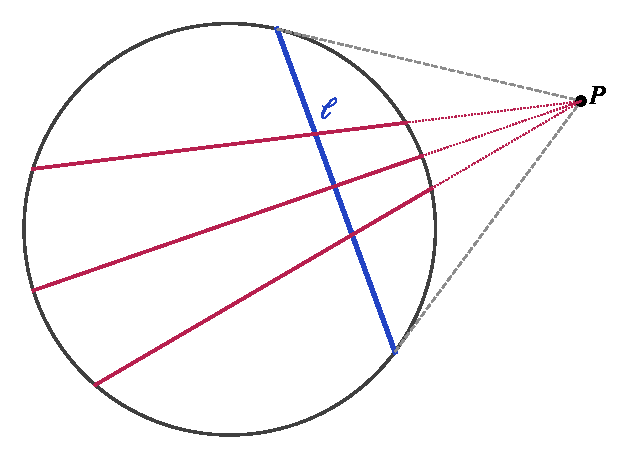
\includegraphics[width=0.5\textwidth]{fig/polyus.pdf}
\caption{Перпендикуляры к π-прямой $\ell$: их продолжения проходят через полюс $P$, точку пересечения касательных к абсолюту в концах хорды $\ell$}
\label{fig:polyus}
\end{figure}

Если $\ell$~--- диаметр, её полюс бесконечно удалён, и лемма говорит, что перпендикуляры к диаметру изображаются хордами, перпендикулярными ему в евклидовом смысле. Этим частным случаем мы будем постоянно пользоваться.

\begin{proposition}\label{prop:ugol}
Пусть π-прямые $\ell_1$ и $\ell_2$ пересекаются, $P_1$ и $P_2$~--- их полюсы, $\varphi$~--- один из углов между ними. Тогда
\begin{equation}\label{eq:ugol}
|\cos\varphi|=\frac{|\sk{P_1}{P_2}|}{\sqrt{\sk{P_1}{P_1}\,\sk{P_2}{P_2}}}.
\end{equation}
\end{proposition}
\begin{proof}
Обе части равенства не меняются при π-движениях, поэтому можно считать, что прямые пересекаются в центре $O$. π-движения, оставляющие $O$ на месте, сохраняют вектор $(1,0,0)$ и форму абсолюта, то есть являются евклидовыми поворотами и симметриями относительно диаметров. Значит, равные углы с вершиной $O$ равны и в евклидовом смысле, а по теореме о единственности меры угла~[2] π-мера угла с вершиной в центре совпадает с евклидовой. Прямые $a_1k_1+a_2k_2=0$ и $b_1k_1+b_2k_2=0$ имеют полюсы $(0:a_1:a_2)$ и $(0:b_1:b_2)$, и правая часть~\eqref{eq:ugol} равна модулю косинуса евклидова угла между нормалями $(a_1,a_2)$ и $(b_1,b_2)$, то есть между самими прямыми.
\end{proof}

Из доказательства видно ещё одно полезное следствие: \emph{угол с вершиной в центре круга изображается без искажения}. Углы с вершиной в другой точке на рисунке искажены, и в интерактивной модели их величина вычисляется по формуле~\eqref{eq:ugol} или, что то же самое, после переноса вершины в центр.

\section{Параллельные и расходящиеся прямые}

\subsection{Параллельные прямые в модели}

Прямые будем считать направленными: направление задаётся упорядоченной парой точек, $a=A_1A_2$.

\begin{definition}[\!\!{[1,~2]}]
Направленная прямая $b=B_1B_2$ называется \emph{параллельной} прямой $a$, если $a$ и $b$ не пересекаются и для любых точек $A\in a$, $B\in b$ любой внутренний луч угла $ABB_2$ пересекает $a$.
\end{definition}

В абсолютной геометрии доказывается~[1], что условие достаточно проверить для одной пары точек $A$, $B$, что через каждую точку вне прямой проходит ровно одна прямая, параллельная ей в данном направлении, и что параллельность симметрична и транзитивна. Модель делает эти утверждения наглядными.

\begin{theorem}\label{thm:parallel-model}
Направленная π-прямая $b=B_1B_2$ параллельна π-прямой $a$ тогда и только тогда, когда конец хорды $b$ в направлении $B_2$ является одним из концов хорды $a$.
\end{theorem}
\begin{proof}
Пусть конец $\Omega$ хорды $b$ в направлении $B_2$ лежит на $a$. Хорды $a$ и $b$ имеют одну общую точку $\Omega$, и она не является π-точкой, поэтому π-прямые не пересекаются. Пусть $A\in a$, $B\in b$ и $h$~--- внутренний луч угла $AB\Omega$. Концы евклидова отрезка $A\Omega$ лежат на сторонах этого угла, поэтому $h$ пересекает отрезок $A\Omega$ во внутренней точке. Эта точка лежит внутри круга и принадлежит $a$.

Обратно, пусть $b$ параллельна $a$, а конец $V$ хорды $b$ в направлении $B_2$ не является концом $a$. Возьмём $A\in a$, $B\in b$. Прямая $AB$ пересекает хорду $a$ в точке $A$, поэтому концы хорды $a$ лежат по разные стороны от прямой $AB$; обозначим через $U$ тот из них, который лежит по одну сторону с $V$. Лучи $BU$ и $BV$ различны. Если луч $BU$ внутренний для угла $ABV$, то он не пересекает $a$ (прямая, содержащая хорду $a$, встречает его только в точке $U$ абсолюта), что противоречит определению. Если же луч $BV$ внутренний для угла $ABU$, то он пересекает отрезок $AU$ во внутренней точке, и прямые $a$ и $b$ пересекаются. Оба случая невозможны.
\end{proof}

Из теоремы~\ref{thm:parallel-model} сразу следуют свойства параллельных, которые в абсолютной геометрии требуют отдельных доказательств~[1]. Через π-точку $B$ вне прямой $a$ проходят ровно две прямые, параллельные $a$: хорды, соединяющие $B$ с концами хорды $a$. Параллельность в фиксированном направлении означает, что хорды имеют один и тот же конец в этом направлении, поэтому она симметрична и транзитивна: если $a$ и $b$ идут в точку $\Omega$ абсолюта, а $b$ и $c$ идут в ту же точку $\Omega$, то и $a$ с $c$ идут в $\Omega$. Для отношения «иметь какой-нибудь общий конец» транзитивность неверна: хорды $\Omega_1\Omega_2$ и $\Omega_1\Omega_3$ имеют общий конец, хорды $\Omega_1\Omega_3$ и $\Omega_3\Omega_4$ тоже, а хорды $\Omega_1\Omega_2$ и $\Omega_3\Omega_4$ его не имеют. Поэтому параллельность всегда рассматривают в определённом направлении. Две различные хорды имеют не больше одного общего конца, поэтому если $A_1A_2\parallel B_1B_2$, то $B_2B_1$ не параллельна $A_2A_1$. Аксиома Лобачевского в модели выполняется: через $B$ проходят по крайней мере две прямые, не пересекающие $a$, и все хорды, лежащие в вертикальных углах между двумя параллельными и не содержащие $a$, тоже её не пересекают.

\subsection{Угол параллельности и формула Лобачевского}

\begin{definition}[\!\!{[1]}]
Пусть $BH$~--- перпендикуляр к прямой $a$, а прямая $b$ проходит через $B$ и параллельна $a$. Угол между лучом $BH$ и прямой $b$ (в направлении параллельности) называется \emph{углом параллельности} отрезка $BH$.
\end{definition}

Равным отрезкам соответствуют равные углы параллельности, поэтому угол параллельности зависит только от длины $x=BH$. Эта зависимость $\Pi(x)$ называется \emph{функцией Лобачевского}. В модели её можно вычислить, если поместить вершину угла в центр круга.

\begin{theorem}\label{thm:lobachevsky}
Для любого $x>0$
\begin{equation}\label{eq:lobachevsky}
\cos\Pi(x)=\thh x,\qquad\text{или, что равносильно,}\qquad \operatorname{tg}\frac{\Pi(x)}{2}=e^{-x}.
\end{equation}
\end{theorem}
\begin{proof}
Переведём π-движением точку $B$ в центр $O$, а точку $H$~--- в точку $(0,-\eta)$ отрицательной полуоси ординат. По следствию~\ref{cor:ot-centra} $\eta=\thh x$. Прямая $a$ перпендикулярна диаметру $BH$ в точке $H$, поэтому по лемме~\ref{lem:polyus} она изображается евклидово перпендикулярной хордой $k_2=-\eta$ с концами $\bigl(\pm\sqrt{1-\eta^2},\,-\eta\bigr)$. Прямые, проходящие через $O$ и параллельные $a$, по теореме~\ref{thm:parallel-model} соединяют $O$ с этими концами. Угол между ними и лучом $OH$ имеет вершину в центре и изображается без искажения (предложение~\ref{prop:ugol}), а его косинус равен
\[
\cos\Pi(x)=\frac{(0,-1)\cdot(\sqrt{1-\eta^2},\,-\eta)}{1}=\eta=\thh x.
\]
Наконец, $\operatorname{tg}^2\frac{\Pi}{2}=\frac{1-\cos\Pi}{1+\cos\Pi}=\frac{1-\thh x}{1+\thh x}=e^{-2x}$.
\end{proof}

\begin{figure}[H]
\centering
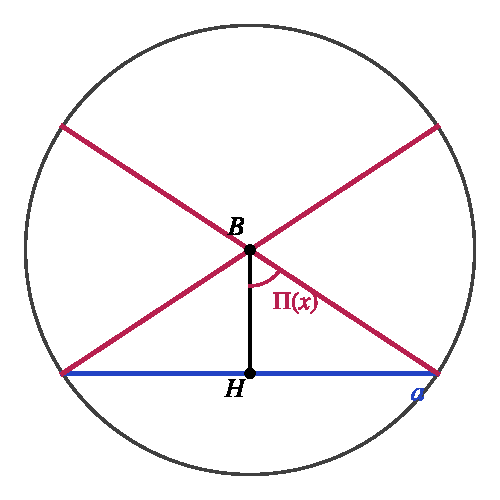
\includegraphics[width=0.46\textwidth]{fig/pi.pdf}
\caption{Угол параллельности отрезка $BH$ при вершине $B$ в центре круга: прямые через $B$, параллельные $a$, идут в концы хорды $a$}
\label{fig:pi}
\end{figure}

Из формулы~\eqref{eq:lobachevsky} видны свойства функции Лобачевского, которые в курсе доказываются с помощью аксиомы Дедекинда. Функция $\Pi(x)$ непрерывна и строго убывает; при $x\to0$ угол стремится к прямому, при $x\to\infty$~--- к нулю. Каждый острый угол $\varphi$ является углом параллельности отрезка длины $x=\operatorname{arth}(\cos\varphi)$. Несколько значений приведены в таблице~\ref{tab:pi}.

\begin{table}[H]
\caption{Значения функции Лобачевского}
\label{tab:pi}
\centering
\begin{tabular}{|c|c|c|c|c|c|}
\hline
$x$ & $0{,}1$ & $0{,}5$ & $1$ & $2$ & $3$ \\ \hline
$\Pi(x)$ & $84{,}28^\circ$ & $62{,}48^\circ$ & $40{,}40^\circ$ & $15{,}41^\circ$ & $5{,}70^\circ$ \\ \hline
\end{tabular}
\end{table}

\subsection{Взаимное расположение двух прямых и общий перпендикуляр}

\begin{definition}[\!\!{[1]}]
Две прямые плоскости Лобачевского называются \emph{расходящимися}, если они не пересекаются и не параллельны.
\end{definition}

Пусть $a$ и $b$~--- различные π-прямые, $X$~--- точка пересечения содержащих их евклидовых прямых (если эти прямые параллельны, $X$~--- бесконечно удалённая точка). По теореме~\ref{thm:parallel-model} прямые $a$ и $b$ пересекаются, если $X$ лежит внутри круга, параллельны, если $X$ лежит на абсолюте, и расходятся, если $X$ лежит вне круга (рисунок~\ref{fig:klassifikaciya}).

\begin{figure}[H]
\centering
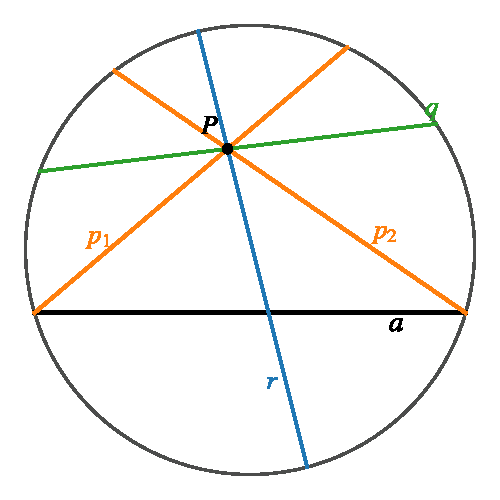
\includegraphics[width=0.48\textwidth]{fig/klassifikaciya.pdf}
\caption{Прямые, проходящие через точку $P$: $r$ пересекает прямую $a$, $p_1$ и $p_2$ ей параллельны, $q$ с ней расходится}
\label{fig:klassifikaciya}
\end{figure}

\begin{theorem}[признак расходящихся прямых]\label{thm:perpendikulyar}
Две непересекающиеся прямые расходятся тогда и только тогда, когда у них есть общий перпендикуляр. Общий перпендикуляр расходящихся прямых единствен; в модели это хорда, проходящая через полюсы обеих прямых.
\end{theorem}
\begin{proof}
Пусть $P_a$ и $P_b$~--- полюсы прямых $a$ и $b$. По лемме~\ref{lem:polyus} прямая перпендикулярна и $a$, и $b$ тогда и только тогда, когда она проходит через $P_a$ и $P_b$, то есть совпадает с евклидовой прямой $P_aP_b$. Точка $X$ лежит на поляре точки $P_a$ (это прямая $a$) и на поляре $P_b$, поэтому по взаимности полюса и поляры прямая $P_aP_b$ есть поляра точки $X$. Если $X$ вне круга, её поляра пересекает круг и даёт единственный общий перпендикуляр. Если $X$ на абсолюте, её поляра~--- касательная, и общего перпендикуляра нет. Если $X$ внутри круга, поляра не пересекает круг; этот случай пересекающихся прямых условием исключён.
\end{proof}

Так в модели выглядит построение общего перпендикуляра: провести касательные к абсолюту в концах обеих хорд, найти два полюса и соединить их. Длину общего перпендикуляра тоже можно найти по полюсам.

\begin{proposition}\label{prop:ch-rasstoyaniya}
Если $a$ и $b$ расходятся, а $\delta$~--- длина их общего перпендикуляра, то
\[
\frac{|\sk{P_a}{P_b}|}{\sqrt{\sk{P_a}{P_a}\sk{P_b}{P_b}}}=\ch\delta.
\]
Для пересекающихся прямых та же величина равна $|\cos\varphi|$ (предложение~\ref{prop:ugol}), для параллельных она равна $1$.
\end{proposition}
\begin{proof}
Величина не меняется при π-движениях. Переведём основание общего перпендикуляра на $a$ в центр, а сам перпендикуляр~--- на ось ординат. Тогда $a$~--- диаметр $k_2=0$ с полюсом $(0:0:1)$, а $b$ перпендикулярна оси ординат и изображается хордой $k_2=c$ с полюсом $(c:0:1)$, где $\delta=\operatorname{arth}|c|$ по следствию~\ref{cor:ot-centra}. Подстановка в~\eqref{eq:forma} даёт $1/\sqrt{1-c^2}=\ch\delta$. Для параллельных прямых поместим общий конец в точку $(1,0)$, а прямую $a$ на диаметр $k_2=0$. Тогда $b$ изображается хордой $\kappa-\kappa k_1-k_2=0$ с полюсом $(\kappa:\kappa:1)$, и $\sk{P_a}{P_b}=1$, $\sk{P_a}{P_a}=1$, $\sk{P_b}{P_b}=-\kappa^2+\kappa^2+1=1$.
\end{proof}

\subsection{Расстояние от точек прямой до другой прямой}

\begin{proposition}\label{prop:do-diametra}
Расстояние $d$ от π-точки $(x,y)$ до диаметра $k_2=0$ определяется равенством
\begin{equation}\label{eq:do-diametra}
\thh d=\frac{|y|}{\sqrt{1-x^2}}.
\end{equation}
\end{proposition}
\begin{proof}
По лемме~\ref{lem:polyus} перпендикуляр из точки $M=(x,y)$ к диаметру изображается вертикальной хордой, его основание $F=(x,0)$. По предложению~\ref{prop:ch}
\[
\ch d(M,F)=\frac{1-x^2}{\sqrt{(1-x^2)(1-x^2-y^2)}}=\sqrt{\frac{1-x^2}{1-x^2-y^2}},
\]
откуда $\thh^2d=1-\dfrac{1}{\ch^2d}=\dfrac{y^2}{1-x^2}$.
\end{proof}

С помощью этой формулы теоремы о расстоянии между точками двух прямых~[1] получают явный вид. Будем двигать точку $M$ по прямой $b$ и следить за её расстоянием до прямой $a$, которую π-движением поместим на диаметр $k_2=0$.

\emph{Параллельные прямые.} Пусть $b$ параллельна $a$ в направлении конца $(1,0)$. Тогда $b$ изображается хордой $y=\kappa(1-x)$, $\kappa\ne0$, и по~\eqref{eq:do-diametra}
\[
\thh d=|\kappa|\,\frac{1-x}{\sqrt{1-x^2}}=|\kappa|\sqrt{\frac{1-x}{1+x}}.
\]
Эта величина строго убывает с ростом $x$, стремится к нулю при $x\to1$ и стремится к единице, то есть $d\to\infty$, когда $M$ уходит к другому концу хорды $b$. Значит, расстояние от точки одной из параллельных прямых до другой неограниченно убывает в направлении параллельности, неограниченно возрастает в противоположном направлении и принимает любое положительное значение ровно один раз.

\emph{Расходящиеся прямые.} Поместим общий перпендикуляр на ось ординат. Прямая $b$ перпендикулярна этой оси и изображается хордой $y=c$, $0<|c|<1$:
\[
\thh d=\frac{|c|}{\sqrt{1-x^2}},\qquad |x|<\sqrt{1-c^2}.
\]
Наименьшее значение $|c|$ достигается при $x=0$, то есть в основании общего перпендикуляра, и равно $\thh\delta$. При удалении $M$ от общего перпендикуляра в любую сторону расстояние неограниченно возрастает (рисунок~\ref{fig:rasstoyanie}).

\begin{figure}[H]
\centering
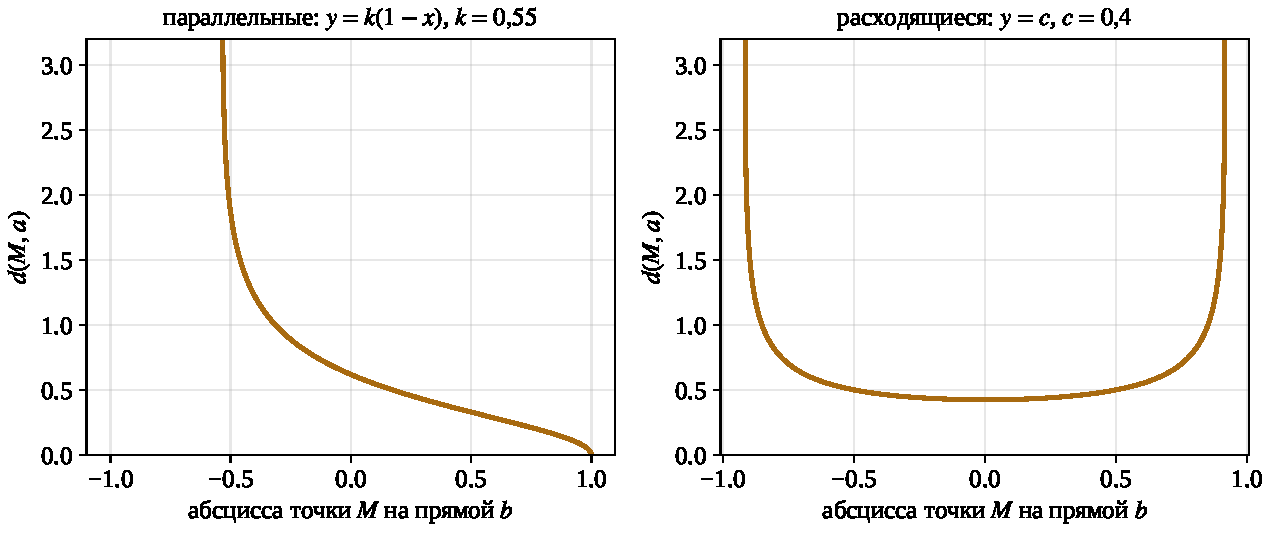
\includegraphics[width=\textwidth]{fig/rasstoyanie.pdf}
\caption{Расстояние от точки $M$ прямой $b$ до прямой $a$ (диаметра $k_2=0$): слева $b$ параллельна $a$, справа расходится с ней}
\label{fig:rasstoyanie}
\end{figure}

В евклидовой геометрии ни того, ни другого поведения нет: точка прямой, параллельной данной, остаётся на одном расстоянии от неё. В интерактивной модели этому посвящена сцена «Общий перпендикуляр и расстояние»: при перетаскивании концов хорды $b$ график расстояния переходит от U-образной кривой к монотонной в тот момент, когда концы хорд совпадают.

\section{Треугольники и четырёхугольники}

В абсолютной геометрии доказывается ряд утверждений, каждое из которых равносильно аксиоме параллельности Евклида: сумма углов треугольника равна $2d$, точки, равноудалённые от прямой, лежат на прямой (предложение Посидония), перпендикуляр к стороне острого угла пересекает другую сторону (предложение Лежандра), около любого треугольника можно описать окружность~[2]. В геометрии Лобачевского выполняются их отрицания. В этом разделе они доказываются и интерпретируются в модели.

\subsection{Сумма углов треугольника}

\begin{definition}
Четырёхугольник $ABCD$, у которого углы при стороне $AB$ прямые, называется \emph{двупрямоугольником} с основанием $AB$. Если, кроме того, $AD=BC$, он называется \emph{четырёхугольником Саккери}, а сторона $CD$~--- его верхним основанием.
\end{definition}

\begin{lemma}\label{lem:sakkeri-ravny}
В абсолютной геометрии углы четырёхугольника Саккери при верхнем основании равны.
\end{lemma}
\begin{proof}
Прямоугольные треугольники $ABD$ и $BAC$ равны по двум катетам ($AB$ общий, $AD=BC$), поэтому $BD=AC$. Тогда треугольники $ADC$ и $BCD$ равны по трём сторонам, и $\angle ADC=\angle BCD$.
\end{proof}

\begin{lemma}\label{lem:treugolnik-sakkeri}
Для любого треугольника $ABC$ существует четырёхугольник Саккери, сумма углов при верхнем основании которого равна сумме углов треугольника.
\end{lemma}
\begin{proof}
Пусть $M$ и $N$~--- середины сторон $AB$ и $AC$. Опустим на прямую $MN$ перпендикуляры $AA'$, $BB'$, $CC'$. Прямоугольные треугольники $AA'M$ и $BB'M$ равны по гипотенузе и острому углу, поэтому $BB'=AA'$ и $\angle B'BM=\angle A'AM$. Точно так же $CC'=AA'$ и $\angle C'CN=\angle A'AN$. Значит, $B'C'CB$~--- четырёхугольник Саккери с основанием $B'C'$. Если точка $A'$ лежит между $B'$ и $C'$, то
\[
\angle B'BC+\angle C'CB=(\angle A'AB+\angle B)+(\angle A'AC+\angle C)=\angle A+\angle B+\angle C.
\]
Остальные случаи расположения точки $A'$ разбираются так же, только одно из слагаемых $\angle A'AB$, $\angle A'AC$ входит со знаком минус.
\end{proof}

Нам понадобятся две теоремы абсолютной геометрии, доказательства которых приведены в~[2].

\begin{theorem}[первая теорема Лежандра]\label{thm:lezhandr1}
Сумма углов любого треугольника не превосходит $2d$.
\end{theorem}

\begin{theorem}[вторая теорема Лежандра]\label{thm:lezhandr2}
Если сумма углов хотя бы одного треугольника равна $2d$, то выполняется аксиома параллельности Евклида.
\end{theorem}

\begin{lemma}\label{lem:sakkeri-ostrye}
В геометрии Лобачевского углы четырёхугольника Саккери при верхнем основании острые.
\end{lemma}
\begin{proof}
Диагональ делит четырёхугольник на два треугольника, поэтому по теореме~\ref{thm:lezhandr1} сумма его углов не больше $4d$. Углы при основании прямые, углы при верхнем основании по лемме~\ref{lem:sakkeri-ravny} равны, значит, каждый из них не больше $d$. Если бы они были прямыми, то диагональ разбила бы прямоугольник на два треугольника с общей суммой углов $4d$, и по теореме~\ref{thm:lezhandr1} сумма углов каждого была бы равна $2d$. По теореме~\ref{thm:lezhandr2} это противоречит аксиоме Лобачевского.
\end{proof}

\begin{theorem}\label{thm:summa}
На плоскости Лобачевского сумма углов любого треугольника меньше $2d$.
\end{theorem}
\begin{proof}
По лемме~\ref{lem:treugolnik-sakkeri} сумма углов треугольника равна сумме двух углов при верхнем основании некоторого четырёхугольника Саккери, а по лемме~\ref{lem:sakkeri-ostrye} каждый из этих углов меньше $d$.
\end{proof}

Число $\delta=2d-(\alpha+\beta+\gamma)$ называется \emph{дефектом} треугольника. Площадь треугольника пропорциональна дефекту~[4]; при выбранной единице длины, когда радиус кривизны равен $1$, площадь равна $\delta$. Отсюда площадь любого треугольника меньше $\pi$. Из леммы~\ref{lem:sakkeri-ostrye} следует, что на плоскости Лобачевского нет прямоугольников, а из теоремы~\ref{thm:summa}~--- что треугольники с соответственно равными углами равны~[1]. Подобных, но не равных фигур в геометрии Лобачевского нет.

\subsection{Четырёхугольник Саккери в модели}

Поместим основание четырёхугольника Саккери на горизонтальный диаметр симметрично относительно центра: $A=(-p,0)$, $B=(p,0)$. По лемме~\ref{lem:polyus} перпендикуляры к диаметру в точках $A$ и $B$ изображаются вертикальными хордами, поэтому $D=(-p,q)$ и $C=(p,q)$ (рисунок~\ref{fig:sakkeri}). Обозначим длину основания через $b$, а длину боковых сторон через $h$. По следствию~\ref{cor:ot-centra} $p=\thh(b/2)$, а по формуле~\eqref{eq:do-diametra} $\thh h=q/\sqrt{1-p^2}$.

\begin{figure}[H]
\centering
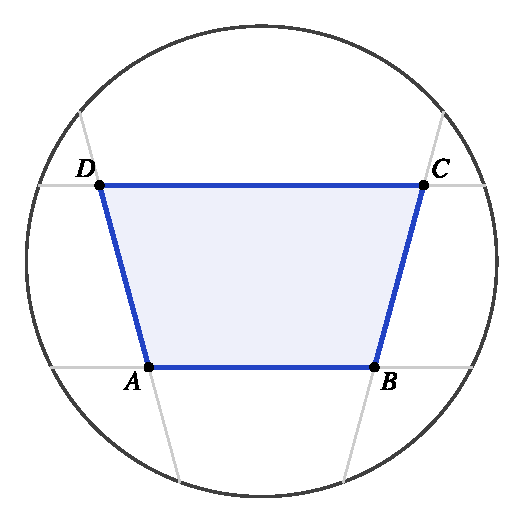
\includegraphics[width=0.46\textwidth]{fig/sakkeri.pdf}
\caption{Четырёхугольник Саккери в модели, перенесённый π-движением вниз. На рисунке он выглядит евклидовой трапецией, углы при верхнем основании равны $54{,}3^\circ$ ($b=1{,}2$, $h=1{,}1$)}
\label{fig:sakkeri}
\end{figure}

\begin{proposition}\label{prop:sakkeri}
Угол $\gamma$ четырёхугольника Саккери при верхнем основании находится по формуле
\begin{equation}\label{eq:sakkeri}
\cos\gamma=\frac{\sh\frac b2\,\sh h}{\sqrt{\ch^2\frac b2+\sh^2\frac b2\,\sh^2h}}.
\end{equation}
\end{proposition}
\begin{proof}
Прямая $BC$ имеет уравнение $k_1-p=0$ и полюс $P_1=(p:1:0)$, прямая $CD$~--- уравнение $k_2-q=0$ и полюс $P_2=(q:0:1)$. По предложению~\ref{prop:ugol}
\[
|\cos\gamma|=\frac{pq}{\sqrt{(1-p^2)(1-q^2)}}.
\]
Угол $\gamma$ острый (лемма~\ref{lem:sakkeri-ostrye}), поэтому знак модуля можно снять. Подставим $p=\thh\frac b2$ и $q=\thh h/\ch\frac b2$; после умножения числителя и знаменателя на $\ch\frac b2\,\ch h$ и замены $\ch^2h=1+\sh^2h$ получается~\eqref{eq:sakkeri}.
\end{proof}

Формула показывает больше, чем утверждение об остроте углов. При $b\to0$ или $h\to0$ угол $\gamma$ стремится к прямому: маленький четырёхугольник Саккери почти неотличим от прямоугольника. При $h\to\infty$ угол стремится к нулю. Числа на рисунке~\ref{fig:sakkeri} получены по этой формуле и совпадают с тем, что показывает сцена «Двупрямоугольник и четырёхугольник Саккери» интерактивной модели.

\subsection{Точки, равноудалённые от прямой}

\begin{definition}[\!\!{[1]}]
Множество точек одной полуплоскости, удалённых от её граничной прямой $a$ на одно и то же расстояние $h$, называется \emph{эквидистантой} с базой $a$ и высотой $h$.
\end{definition}

\begin{proposition}\label{prop:ekvidistanta}
Если база~--- диаметр $k_2=0$, эквидистанта высоты $h$ изображается дугой эллипса
\[
y=\thh h\,\sqrt{1-x^2},\qquad |x|<1,
\]
с полуосями $1$ и $\thh h$. Она не является прямой.
\end{proposition}
\begin{proof}
Уравнение получается из~\eqref{eq:do-diametra}, если положить $d=h$ и $y>0$. Три её точки с абсциссами $0$ и $\pm\frac12$ не лежат на одной хорде: средняя расположена выше хорды, соединяющей крайние, так как функция $\sqrt{1-x^2}$ строго вогнута.
\end{proof}

Это интерпретация отрицания предложения Посидония (рисунок~\ref{fig:ekvidistanta}). Концы эквидистанты совпадают с концами базы, поэтому эквидистанта, в отличие от прямой, параллельной базе, не уходит от неё и не приближается к ней.

\begin{figure}[H]
\centering
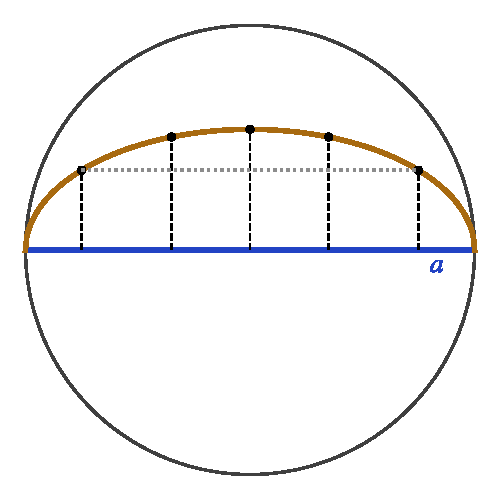
\includegraphics[width=0.46\textwidth]{fig/ekvidistanta.pdf}
\caption{Эквидистанта высоты $0{,}6$ с базой $a$ и перпендикуляры к базе равной длины; пунктир~--- хорда через две точки эквидистанты}
\label{fig:ekvidistanta}
\end{figure}

\subsection{Перпендикуляр к стороне острого угла}

\begin{proposition}\label{prop:lezhandr}
Пусть угол $E_1OE_2$ острый и равен $\varphi$, $P$~--- точка на стороне $OE_1$, $x=OP$. Перпендикуляр к $OE_1$ в точке $P$ пересекает сторону $OE_2$ тогда и только тогда, когда $\Pi(x)>\varphi$. Граничная точка $P^*$, для которой $\Pi(OP^*)=\varphi$, существует для любого острого угла, и перпендикуляр в ней параллелен $OE_2$.
\end{proposition}
\begin{proof}
Поместим вершину $O$ в центр, сторону $OE_1$ на положительную полуось абсцисс, сторону $OE_2$ на луч $t(\cos\varphi,\sin\varphi)$, $0\le t<1$. Угол с вершиной в центре изображается без искажения. По следствию~\ref{cor:ot-centra} точка $P$ изображается точкой $(\thh x,0)$, и по лемме~\ref{lem:polyus} перпендикуляр в ней изображается вертикальной хордой $k_1=\thh x$. Луч $OE_2$ пересекает прямую $k_1=\thh x$ в точке с параметром $t=\thh x/\cos\varphi$, и эта точка лежит в круге тогда и только тогда, когда $\thh x<\cos\varphi$. По теореме~\ref{thm:lobachevsky} $\thh x=\cos\Pi(x)$, поэтому условие равносильно $\Pi(x)>\varphi$. При $\thh x=\cos\varphi$ хорда $k_1=\thh x$ проходит через конец $E_2=(\cos\varphi,\sin\varphi)$ стороны $OE_2$ и по теореме~\ref{thm:parallel-model} параллельна ей.
\end{proof}

Получилось отрицание предложения Лежандра (рисунок~\ref{fig:lezhandr}) и одновременно ещё одно доказательство того, что каждый острый угол является углом параллельности некоторого отрезка. В курсе эти два факта связаны так же: существование отрезка с данным углом параллельности выводится из отрицания предложения Лежандра.

\begin{figure}[H]
\centering
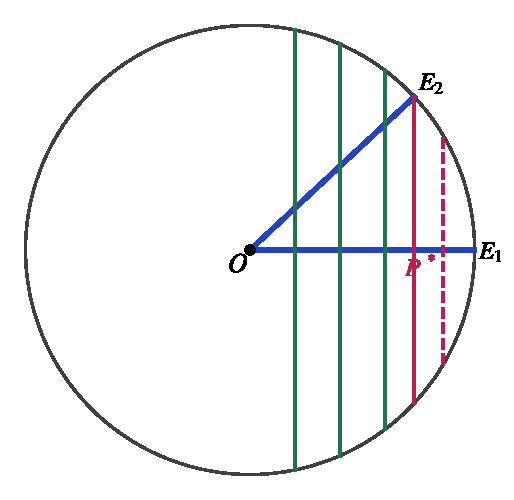
\includegraphics[width=0.46\textwidth]{fig/lezhandr.pdf}
\caption{Перпендикуляры к стороне $OE_1$ острого угла: зелёные пересекают сторону $OE_2$, красный проходит через её конец $E_2$ и ей параллелен, пунктирный её не пересекает}
\label{fig:lezhandr}
\end{figure}

Здесь же видно и отрицание V постулата: прямая $OE_2$ и перпендикуляр в точке $P^*$ не пересекаются, хотя образуют с прямой $OE_1$ внутренние односторонние углы $\varphi$ и $d$, сумма которых меньше $2d$.

\subsection{Треугольник без описанной окружности}

Центр окружности, описанной около треугольника, лежит на серединных перпендикулярах к его сторонам. Поэтому треугольник, у которого два серединных перпендикуляра не пересекаются, окружности не имеет. Пример строится так~[1]. Пусть $a$~--- прямая, $h$~--- перпендикуляр к ней, $A\in h$, и $b$~--- прямая через $A$, не перпендикулярная $h$ и не пересекающая $a$; по теореме~\ref{thm:lv-vsegda} такая прямая существует. Возьмём точку $M\in h$ и отразим её относительно $a$ и $b$, получим точки $N$ и $P$. Тогда $a$ и $b$~--- серединные перпендикуляры к сторонам $MN$ и $MP$ треугольника $MNP$, и они не пересекаются.

В модели все построения выполняются по формулам п.~1.4. На рисунке~\ref{fig:bez-okruzhnosti} прямая $a$~--- горизонтальный диаметр, $h$~--- вертикальный, а прямая $b$ выбрана так, что продолжения хорд $a$ и $b$ пересекаются вне круга; точки $N$ и $P$ получены по формуле~\eqref{eq:otrazhenie}.

\begin{figure}[H]
\centering
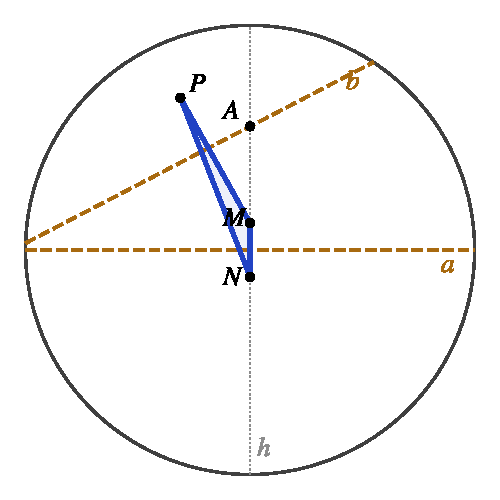
\includegraphics[width=0.46\textwidth]{fig/bez_okruzhnosti.pdf}
\caption{Треугольник $MNP$, серединные перпендикуляры $a$ и $b$ которого расходятся}
\label{fig:bez-okruzhnosti}
\end{figure}

Если же две прямые пересекаются, то любая точка, не лежащая на них, отражённая относительно обеих прямых, даёт треугольник, около которого окружность описать можно.

\section{Модель и аксиоматика}

\subsection{Непротиворечивость}

Интерпретацией системы аксиом называется выбор конкретных множеств и отношений на них в качестве основных понятий. Если в интерпретации выполнены все аксиомы, она называется моделью системы~[3]. Модель Кэли~--- Клейна построена средствами евклидовой геометрии: её точки, прямые и движения~--- евклидовы точки, хорды и проективные преобразования, сохраняющие окружность. В разделах~1 и~2 проверено, что в ней выполняются аксиомы I--IV групп и аксиома Лобачевского.

Отсюда следует, что геометрия Лобачевского непротиворечива, если непротиворечива геометрия Евклида. Действительно, если бы из аксиом Лобачевского выводились утверждение и его отрицание, то, переводя вывод на язык модели, мы получили бы противоречие в евклидовой геометрии. Такая непротиворечивость называется относительной~[3,~8]: модель не доказывает, что геометрия Лобачевского свободна от противоречий сама по себе, она показывает, что эта геометрия не может оказаться противоречивой раньше, чем евклидова.

\subsection{Независимость аксиомы параллельности}

Аксиома $A$ называется независимой от системы аксиом $\Sigma$, если ни $A$, ни её отрицание не выводятся из $\Sigma$. Чтобы это доказать, достаточно предъявить две модели системы $\Sigma$: в одной $A$ выполняется, в другой нет~[3].

Для аксиомы параллельности Евклида и системы аксиом I--IV такими моделями служат евклидова плоскость и модель Кэли~--- Клейна. На евклидовой плоскости через точку вне прямой проходит ровно одна прямая, не пересекающая данную. В модели таких прямых бесконечно много (п.~2.1). Если бы аксиома параллельности выводилась из I--IV, она была бы верна в обеих моделях. Если бы выводилось её отрицание, оно тоже было бы верно в обеих. Значит, аксиома параллельности не зависит от аксиом I--IV. Именно поэтому двухтысячелетние попытки вывести V постулат из остальных аксиом не могли закончиться успехом.

\subsection{Что модель показывает и чего не доказывает}

Модель отвечает на вопрос, что означает утверждение геометрии Лобачевского, и позволяет проверить его на сколь угодно многих конкретных фигурах. Например, сумма углов треугольника, вычисленная в модели для любого положения вершин, оказывается меньше $2d$. Однако никакое число таких проверок не заменяет доказательства: модель лишь одна из интерпретаций, и рассуждение, опирающееся на свойства хорд или на вид рисунка, может использовать то, чего нет в аксиомах. Поэтому в разделах~1--3 каждое утверждение сначала доказывается средствами абсолютной геометрии или ссылкой на~[1,~2], а модель используется для интерпретации и для вычисления величин.

Есть и обратная польза. В модели легко увидеть, какое утверждение верно, прежде чем его доказывать. Если медленно передвигать конец одной из двух хорд, видно, как пересекающиеся прямые становятся параллельными, затем расходящимися, и как в этот момент появляется общий перпендикуляр, который сначала уходит к абсолюту, а затем возвращается. Такое наблюдение становится гипотезой, а доказательство затем проводится по аксиомам. В интерактивной модели рядом с каждым рисунком приведена формулировка утверждения, а вопросы к сцене предлагают сначала предсказать результат и только потом проверить его на рисунке.

\section{Пучки прямых, связки и простейшие поверхности}

Этот и следующий разделы расширяют предыдущие: те же средства модели~--- форма абсолюта, полюсы, симметрии~--- применяются к пучкам прямых и их траекториям, а затем к пространству.

\subsection{Нормированные координаты}

Однородные координаты точки определены с точностью до множителя. Для π-точки $k$ выберем представителя
\begin{equation}\label{eq:norm}
X=\frac{(1,k)}{\sqrt{1-|k|^2}},\qquad \sk{X}{X}=-1,\quad x_0>0,
\end{equation}
и назовём его \emph{нормированным вектором} точки. Для внешней точки $P$ (полюса прямой) нормированным будем называть представителя с $\sk{P}{P}=1$. В нормированных координатах формулы раздела~1 упрощаются: по предложению~\ref{prop:ch} $\ch d(X,Y)=-\sk{X}{Y}$, а расстояние от точки $X$ до прямой с нормированным полюсом $P$ равно
\begin{equation}\label{eq:do-pryamoy}
\sh d=|\sk{X}{P}|.
\end{equation}
Для доказательства переведём прямую π-движением на диаметр $k_2=0$ с полюсом $(0:0:1)$; при $X=(1,x,y)/\sqrt{1-x^2-y^2}$ равенство~\eqref{eq:do-pryamoy} совпадает с~\eqref{eq:do-diametra}, переписанным через $\sh d=\thh d/\sqrt{1-\thh^2 d}$.

Наконец, если точка движется по кривой и $X(t)$~--- её нормированный вектор, то из $\ch d=-\sk{X(t)}{X(t+\Delta t)}$ и равенства $\sk{X}{X}=-1$ получается, что элемент длины кривой равен $ds^2=\sk{dX}{dX}$, а касательные векторы $u$ удовлетворяют условию $\sk{u}{X}=0$. Угол между двумя кривыми в общей точке измеряется формой $\sk{\cdot}{\cdot}$ на их касательных векторах; для прямых это согласуется с предложением~\ref{prop:ugol}.

\subsection{Пучки прямых и их траектории}

\begin{definition}[\!\!{[1]}]
\emph{Пучком пересекающихся прямых} называется множество всех прямых, проходящих через точку (центр пучка). \emph{Пучком параллельных прямых} называется множество всех прямых, параллельных данной прямой в данном направлении. \emph{Пучком расходящихся прямых} называется множество всех прямых, перпендикулярных данной прямой (базе пучка).
\end{definition}

\begin{proposition}\label{prop:puchok}
Каждый пучок совпадает с множеством $B_V$ π-прямых, содержащие которые евклидовы прямые проходят через фиксированную точку $V$ проективной плоскости. Для пучка пересекающихся прямых $V$~--- центр пучка (внутренняя точка), для пучка параллельных~--- общий конец прямых (точка абсолюта), для пучка расходящихся~--- полюс базы (внешняя точка).
\end{proposition}
\begin{proof}
Первое утверждение очевидно, второе следует из теоремы~\ref{thm:parallel-model}, третье~--- из леммы~\ref{lem:polyus}.
\end{proof}

Через любую π-точку $A$, отличную от центра пучка, проходит ровно одна прямая пучка: это прямая $AV$. Точку $A$ называют \emph{обыкновенной}, если она не является центром пучка и не лежит на базе~[1].

\begin{definition}[\!\!{[1]}]
\emph{Траекторией} обыкновенной точки $A$ относительно пучка называется множество точек, симметричных $A$ относительно прямых пучка.
\end{definition}

\begin{theorem}\label{thm:traektoriya}
Пусть пучок задан точкой $V$ (с фиксированным представителем), $A$~--- его обыкновенная точка. Траектория точки $A$ есть множество π-точек, нормированные векторы которых удовлетворяют условию
\[
\sk{X}{V}=\sk{A}{V}.
\]
\end{theorem}
\begin{proof}
Пусть $X=\sigma_\ell(A)$, где $\ell$~--- прямая пучка с полюсом $P$. Так как $V$ лежит на $\ell$, то $\sk{V}{P}=0$ и по формуле~\eqref{eq:otrazhenie} $\sigma_\ell(V)=V$. Симметрия сохраняет форму абсолюта и переводит нормированные векторы в нормированные: она непрерывна и оставляет на месте точки прямой $\ell$. Поэтому $\sk{X}{V}=\sk{\sigma_\ell A}{\sigma_\ell V}=\sk{A}{V}$.

Обратно, пусть $\sk{B}{V}=\sk{A}{V}$ и $B\ne A$. Положим $m=A-B$. Тогда
\[
\sk{m}{m}=-2-2\sk{A}{B}=2\bigl(\ch d(A,B)-1\bigr)>0,
\]
то есть $m$~--- внешняя точка, и её поляра $\ell$ является π-прямой. Так как $\sk{A}{m}=-1-\sk{A}{B}=\tfrac12\sk{m}{m}$, по формуле~\eqref{eq:otrazhenie}
\[
\sigma_\ell(A)=A-\frac{2\sk{A}{m}}{\sk{m}{m}}\,m=A-m=B.
\]
Наконец, $\sk{m}{V}=\sk{A}{V}-\sk{B}{V}=0$, то есть $V$ лежит на поляре $\ell$ точки $m$, и прямая $\ell$ принадлежит пучку. Точка $B=A$ получается симметрией относительно прямой пучка, проходящей через $A$.
\end{proof}

Прямая $\ell$ из доказательства~--- серединный перпендикуляр к отрезку $AB$, а её полюс~--- точка $A-B$. Три типа пучков различаются только положением точки $V$, и разбирать их отдельно не понадобилось.

\begin{corollary}\label{cor:traektorii}
Траектория относительно пучка пересекающихся прямых~--- окружность с центром $V$; относительно пучка расходящихся прямых~--- эквидистанта с базой, полярной точке $V$ (по формуле~\eqref{eq:do-pryamoy}); относительно пучка параллельных прямых~--- кривая, которая называется \emph{орициклом}.
\end{corollary}

Подставляя~\eqref{eq:norm} в условие $\sk{X}{V}=c$, где $V=(v_0,\bar v)$, получаем уравнение траектории в координатах круга:
\begin{equation}\label{eq:klein-traektoriya}
(k\cdot\bar v-v_0)^2=c^2\,(1-|k|^2).
\end{equation}
Это кривая второго порядка, и при всех трёх типах пучков она изображается эллипсом или его дугой. Для окружности с центром $q$ и радиусом $\rho$ уравнение имеет вид $(1-k\cdot q)^2=\ch^2\rho\,(1-|q|^2)(1-|k|^2)$; для орицикла с концом $\omega$ на абсолюте~--- $(1-k\cdot\omega)^2=c^2(1-|k|^2)$; для эквидистанты к хорде $k\cdot e=\sigma$ ($|e|=1$, $|\sigma|<1$)~--- $(k\cdot e-\sigma)^2=\sh^2h\,(1-\sigma^2)(1-|k|^2)$. Орицикл касается абсолюта в точке $\omega$, эквидистанта подходит к абсолюту в концах базы, окружность лежит строго внутри круга (рисунок~\ref{fig:puchki}).

\begin{figure}[H]
\centering
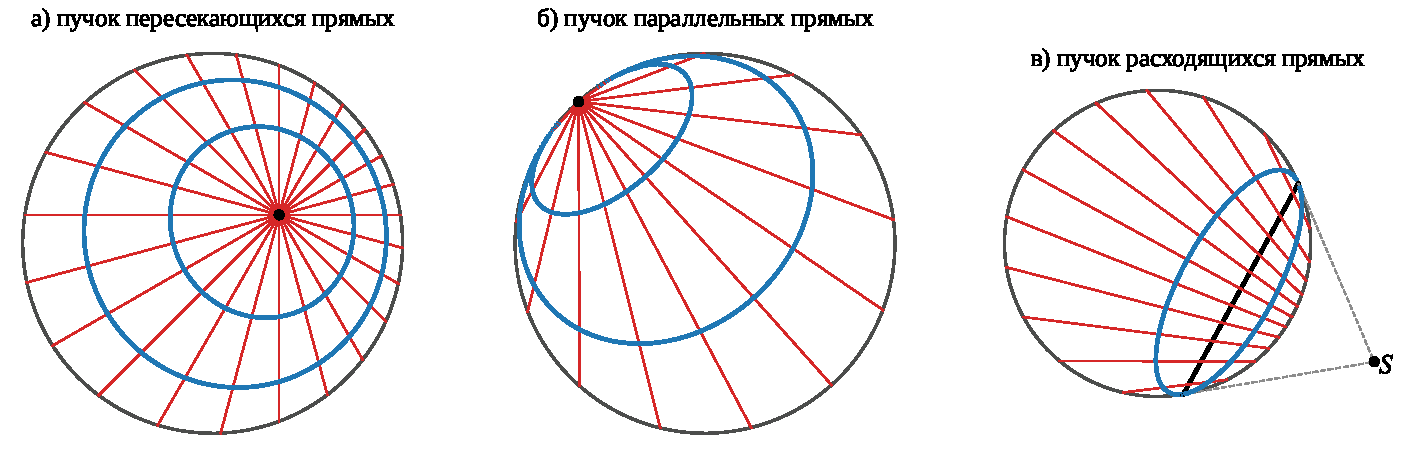
\includegraphics[width=\textwidth]{fig/puchki.pdf}
\caption{Пучки прямых (красные хорды) и их траектории (синие кривые). В случае в) продолжения хорд пучка проходят через полюс $S$ базы (чёрная хорда), синие кривые~--- эквидистанты по обе стороны от базы}
\label{fig:puchki}
\end{figure}

\subsection{Пространство Лобачевского в модели}

Модель пространства устроена так же, как модель плоскости. Абсолютом служит единичная сфера, π-точками~--- внутренние точки шара, π-прямыми~--- хорды, π-плоскостями~--- сечения шара евклидовыми плоскостями, которые его пересекают. Форма абсолюта в однородных координатах $(x_0:x_1:x_2:x_3)$ имеет вид $\sk{X}{Y}=-x_0y_0+x_1y_1+x_2y_2+x_3y_3$. Каждая π-плоскость есть поляра внешней точки, своего полюса; формулы~\eqref{eq:ch}, \eqref{eq:otrazhenie}, \eqref{eq:norm} и~\eqref{eq:do-pryamoy} сохраняются, только $\sigma$ теперь~--- симметрия относительно плоскости, а~\eqref{eq:do-pryamoy} даёт расстояние до плоскости. Повторяя доказательство леммы~\ref{lem:polyus}, получаем: \emph{прямая перпендикулярна плоскости тогда и только тогда, когда продолжение хорды проходит через полюс плоскости}. Проходить через центр шара π-плоскость не обязана.

Две прямые пространства, не лежащие в одной плоскости, называются \emph{скрещивающимися}. Прямые одной плоскости пересекаются, параллельны или расходятся (раздел~2). Расходящиеся и скрещивающиеся прямые имеют единственный общий перпендикуляр~[1]. Две плоскости с нормированными полюсами $P_1$, $P_2$ пересекаются по прямой, если $|\sk{P_1}{P_2}|<1$, параллельны (имеют одну общую точку абсолюта), если $|\sk{P_1}{P_2}|=1$, и расходятся, если $|\sk{P_1}{P_2}|>1$; в последнем случае прямая $P_1P_2$ даёт их единственный общий перпендикуляр. Доказательство повторяет рассуждения п.~2.3.

\subsection{Связки прямых и пучки плоскостей}

\begin{definition}[\!\!{[1]}]
\emph{Связкой пересекающихся прямых} называется множество всех прямых, проходящих через точку $O$. \emph{Связкой параллельных прямых} называется множество всех прямых, параллельных данной прямой в данном направлении. \emph{Связкой расходящихся прямых} называется множество всех прямых, перпендикулярных данной плоскости (базе связки).
\end{definition}

Третью связку не следует путать с пучком расходящихся прямых: прямые одной плоскости, перпендикулярные одной прямой, образуют пучок, и поверхности, перпендикулярной всем им, в пространстве нет.

\begin{proposition}\label{prop:svyazka}
Каждая связка совпадает с множеством $B_V$ π-прямых, продолжения которых проходят через фиксированную точку $V$: внутреннюю для связки пересекающихся прямых, лежащую на абсолюте для связки параллельных и внешнюю (полюс базы) для связки расходящихся.
\end{proposition}
\begin{proof}
Первые два случая разбираются так же, как в предложении~\ref{prop:puchok}, третий следует из описания перпендикуляра к плоскости.
\end{proof}

\emph{Пучок плоскостей}~--- это множество π-плоскостей, содержащих одну евклидову прямую $u$. Если $u$ пересекает шар, это все плоскости, проходящие через π-прямую. Если $u$ касается абсолюта в точке $\omega$, все плоскости пучка проходят через $\omega$ и попарно параллельны. Если $u$ лежит вне шара, все плоскости пучка перпендикулярны одной π-прямой, полярной прямой $u$: плоскость с полюсом $P$ перпендикулярна прямой тогда и только тогда, когда продолжение этой прямой проходит через $P$.

\subsection{Простейшие поверхности как траектории связок}

Плоскость, проходящую через точку $V$, назовём \emph{плоскостью связки} $B_V$. Каждая плоскость связки состоит из прямых связки.

\begin{theorem}\label{thm:svyazka}
Пусть связка задана точкой $V$, $c$~--- число, и множество
\[
S=\{X:\ \sk{X}{X}=-1,\ x_0>0,\ \sk{X}{V}=c\}
\]
непусто и не содержит центра связки. Тогда:
\begin{enumerate}
  \item через каждую точку $X\in S$ проходит ровно одна прямая связки, и она перпендикулярна поверхности $S$;
  \item связная поверхность, перпендикулярная всем прямым связки, которые она пересекает, целиком лежит на одной из поверхностей $S$;
  \item $S$~--- множество точек, симметричных фиксированной точке $A\in S$ относительно плоскостей связки;
  \item пересечение $S$ с любой плоскостью связки~--- траектория соответствующего пучка прямых в этой плоскости.
\end{enumerate}
\end{theorem}
\begin{proof}
1. Касательные векторы $u$ к поверхности $S$ в точке $X$ удовлетворяют условиям $\sk{u}{X}=0$ и $\sk{u}{V}=0$. Прямая связки через $X$ лежит в евклидовой плоскости, натянутой на векторы $X$ и $V$ (они не пропорциональны, так как $X$ не центр). Её касательный вектор в точке $X$ получается из $V$ вычитанием составляющей вдоль $X$:
\[
w=V+\sk{X}{V}\,X,\qquad \sk{w}{X}=\sk{X}{V}-\sk{X}{V}=0.
\]
Для любого касательного вектора $u$ к $S$ имеем $\sk{u}{w}=\sk{u}{V}+\sk{X}{V}\sk{u}{X}=0$, то есть прямая перпендикулярна $S$.

2. Вектор $w$ направлен по градиенту функции $f(X)=\sk{X}{V}$ на множестве нормированных векторов. Если поверхность перпендикулярна всем прямым связки, производная $f$ вдоль неё равна нулю, и на связной поверхности $f$ постоянна.

3. Для плоскости связки с полюсом $P$ выполнено $\sk{V}{P}=0$, симметрия оставляет $V$ на месте и сохраняет $f$. Обратное включение доказывается теми же выкладками с вектором $m=A-B$, что и в теореме~\ref{thm:traektoriya}.

4. На плоскости связки $\Sigma$ форма абсолюта индуцирует форму абсолюта этой плоскости, точка $V$ задаёт в ней пучок, и $S\cap\Sigma$ описывается тем же уравнением $\sk{X}{V}=c$. По теореме~\ref{thm:traektoriya} это траектория пучка.
\end{proof}

\begin{corollary}\label{cor:poverhnosti}
\begin{enumerate}
  \item Если $V=O$~--- внутренняя точка, то $S$ при $c=-\ch\rho$~--- \emph{сфера} с центром $O$ радиуса $\rho$. Её сечение плоскостью, проходящей через центр,~--- окружность того же радиуса.
  \item Если $V=\ell$~--- точка абсолюта, то $S$~--- \emph{орисфера}. Её сечение плоскостью, проходящей через $\ell$,~--- орицикл.
  \item Если $V=P$~--- полюс плоскости $\Pi$, то $S$ при $c=\sh h$~--- \emph{эквидистантная поверхность}, множество точек одной стороны от $\Pi$, удалённых от неё на $h$. Её сечение плоскостью, перпендикулярной $\Pi$,~--- эквидистанта.
\end{enumerate}
\end{corollary}

Утверждения о том, что сфера, орисфера и эквидистантная поверхность ортогональны соответствующим связкам, получают одно общее доказательство.

\subsection{Изображение поверхностей в модели}

Подставим $X=(1,k)/\sqrt{1-|k|^2}$, $k\in\R^3$, $|k|<1$, в уравнение $\sk{X}{V}=c$:
\begin{equation}\label{eq:klein-poverhnost}
(k\cdot\bar v-v_0)^2=c^2\,(1-|k|^2),\qquad V=(v_0,\bar v).
\end{equation}
Это поверхность второго порядка, квадратичная часть $(k\cdot\bar v)^2+c^2|k|^2$ положительно определена, поэтому все три поверхности изображаются эллипсоидами или их частями.

\begin{remark}
Уравнение~\eqref{eq:klein-poverhnost} имеет вид $F_1^2-c^2F_2=0$, где $F_2=0$~--- уравнение абсолюта, а $F_1=0$~--- уравнение плоскости, полярной точке $V$~[7]. Значит, все три поверхности принадлежат пучку квадрик, порождённому абсолютом и сдвоенной полярной плоскостью точки $V$, и касаются абсолюта вдоль сечения этой плоскостью. Для сферы полярная плоскость центра лежит вне шара, и касание мнимое; для орисферы это касательная плоскость в точке $\ell$; для эквидистантной поверхности это сама база $\Pi$, и поверхность подходит к абсолюту по окружности, по которой его пересекает база.
\end{remark}

\textbf{Сфера.} Пусть центр изображается точкой $q$, $a=|q|<1$, радиус равен $\rho$, $C=\ch^2\rho$. Уравнение~\eqref{eq:klein-poverhnost} принимает вид $(1-k\cdot q)^2=C(1-a^2)(1-|k|^2)$. Направим ось $z$ вдоль $q$ и обозначим через $y$ расстояние от точки до этой оси. Тогда $(1-az)^2=C(1-a^2)(1-z^2-y^2)$. Положим $B=a^2+C(1-a^2)$. Выделяя полный квадрат по $z$, получаем
\[
B\Bigl(z-\frac aB\Bigr)^2+C(1-a^2)\,y^2=\frac{C(C-1)(1-a^2)^2}{B}.
\]
Следовательно, сфера изображается эллипсоидом вращения с осью вдоль $q$, евклидовым центром $q/B$ и полуосями
\begin{equation}\label{eq:sfera-poluosi}
r_\perp=\sqrt{\frac{(1-a^2)(C-1)}{B}},\qquad r_\parallel=\frac{(1-a^2)\sqrt{C(C-1)}}{B}.
\end{equation}
Евклидов центр эллипсоида $q/B$ совпадает с изображением центра сферы только при $q=0$. При $a=0{,}6$ и $\rho=1$ получаем $B\approx1{,}884$, евклидов центр на расстоянии $0{,}318$ от центра шара, $r_\perp\approx0{,}685$, $r_\parallel\approx0{,}616$. При малом $\rho$ имеем $C\approx1$ и $B\approx1$, и евклидов центр почти совпадает с $q$. С ростом радиуса он всё дальше отходит от $q$ к центру шара (рисунок~\ref{fig:sravnenie}).

\begin{figure}[H]
\centering
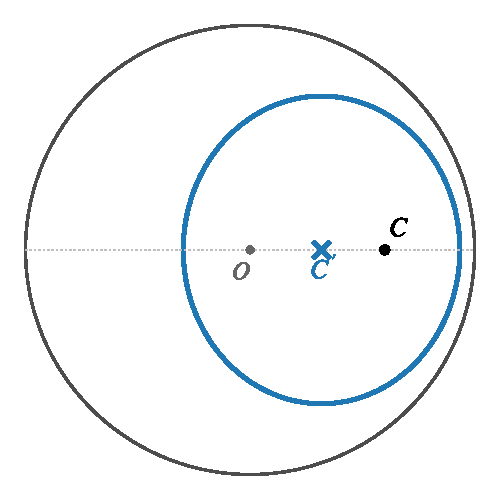
\includegraphics[width=0.46\textwidth]{fig/sravnenie.pdf}
\caption{Сечение сферы с центром $C$ ($a=0{,}6$, $\rho=1$) плоскостью, проходящей через центр шара $O$: эллипс, изображение центра $C$ и евклидов центр эллипса $C'$}
\label{fig:sravnenie}
\end{figure}

\textbf{Орисфера.} Для $\ell=(1,\omega)$, $|\omega|=1$, уравнение~\eqref{eq:klein-poverhnost} даёт $(1-k\cdot\omega)^2=c^2(1-|k|^2)$. Направим ось $z$ вдоль $\omega$; тогда $(1-z)^2=c^2(1-z^2-y^2)$, и после выделения полного квадрата
\[
c^2y^2+(1+c^2)\Bigl(z-\frac1{1+c^2}\Bigr)^2=\frac{c^4}{1+c^2}.
\]
При $r=c/\sqrt{1+c^2}$ это эллипсоид вращения с полуосями $r$ поперёк оси и $r^2$ вдоль неё и с центром $(1-r^2)\omega$, касающийся абсолюта в точке $\omega$. Для сравнения: в модели Пуанкаре орисфера изображается евклидовой сферой, касающейся абсолюта в той же точке.

\textbf{Эквидистантная поверхность} к плоскости $k\cdot e=\sigma$ ($|e|=1$, $|\sigma|<1$) задаётся уравнением $(k\cdot e-\sigma)^2=\sh^2h\,(1-\sigma^2)(1-|k|^2)$. При $\sigma=0$, $e=(0,0,1)$ получаем $z=\pm\thh h\,\sqrt{1-x^2-y^2}$, пространственный аналог предложения~\ref{prop:ekvidistanta}.

На рисунке~\ref{fig:poverhnosti} сфера и орисфера изображены похожими эллипсоидами, и различаются они положением относительно абсолюта. Сфера лежит строго внутри шара: её эллипсоид нигде не касается граничной сферы, а прямые связки сходятся в центре $O$ внутри шара. Орисфера касается абсолюта в точке $\omega$, и все прямые её связки выходят из этой точки, то есть попарно параллельны. Если уводить центр сферы, проходящей через фиксированную точку, к точке $\omega$, сферы стремятся к орисфере; в интерактивной модели этому посвящена сцена «От сферы к орисфере». Эквидистантная поверхность подходит к абсолюту по целой окружности, по той, по которой его пересекает база.

\begin{figure}[H]
\centering
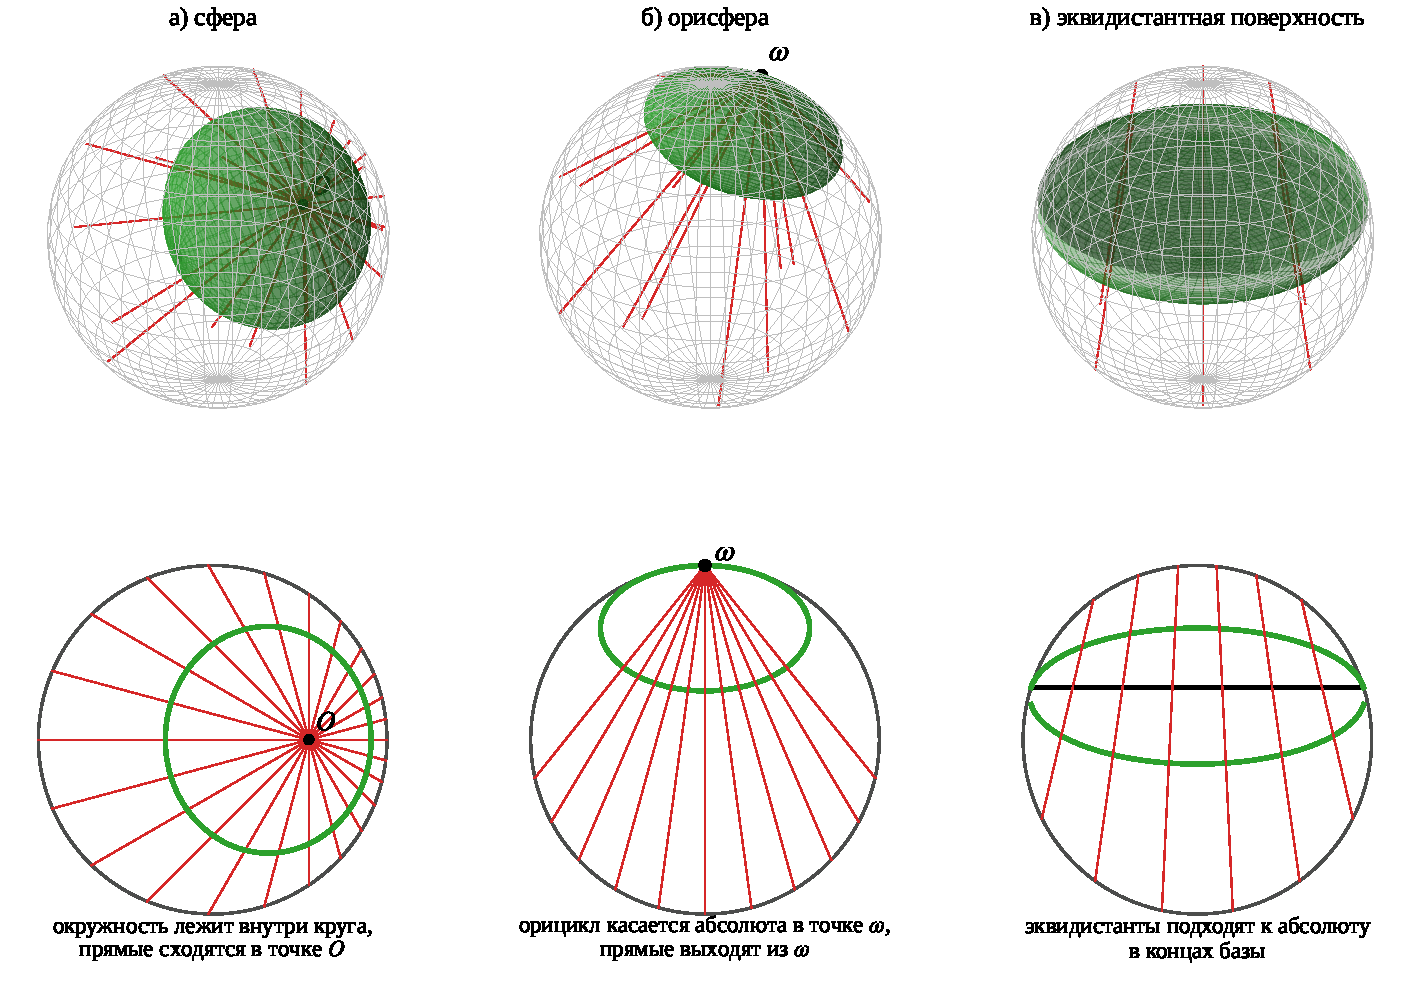
\includegraphics[width=\textwidth]{fig/poverhnosti.pdf}
\caption{Верхний ряд: а) сфера с центром $O$ и прямые собственной связки; б) орисфера и прямые связки параллельных прямых, выходящие из точки $\omega$ абсолюта; в) эквидистантная поверхность к плоскости $z=0{,}3$ и перпендикуляры к этой плоскости, продолжения которых сходятся в её полюсе. Нижний ряд: сечения тех же поверхностей плоскостью, проходящей через центр шара и ось поверхности}
\label{fig:poverhnosti}
\end{figure}

\subsection{Внутренняя геометрия поверхностей}

\begin{theorem}\label{thm:krivizna}
Внутренняя геометрия сферы радиуса $\rho$~--- геометрия евклидовой сферы радиуса $\sh\rho$, её гауссова кривизна равна $1/\sh^2\rho$. Внутренняя геометрия орисферы евклидова. Внутренняя геометрия эквидистантной поверхности на расстоянии $h$ от базы~--- геометрия плоскости Лобачевского с кривизной $-1/\ch^2h$.
\end{theorem}
\begin{proof}
\emph{Сфера.} Нормированные векторы точек сферы с центром $O$ имеют вид $X=\ch\rho\,O+\sh\rho\,u$, где $u$ пробегает векторы с $\sk{u}{O}=0$ и $\sk{u}{u}=1$. На векторах, ортогональных внутренней точке $O$, форма абсолюта положительно определена, то есть задаёт обычное евклидово скалярное произведение. Так как $dX=\sh\rho\,du$ и $ds^2=\sk{dX}{dX}$, длины на сфере в $\sh\rho$ раз больше длин на единичной евклидовой сфере.

\emph{Эквидистантная поверхность.} Каждую её точку можно записать как $X=\ch h\,Y+\sh h\,P$, где $P$~--- нормированный полюс базы, а $Y=(X-\sh h\,P)/\ch h$ лежит на базе: $\sk{Y}{P}=0$ и $\sk{Y}{Y}=-1$. Так как $dX=\ch h\,dY$, метрика поверхности в $\ch^2h$ раз больше метрики плоскости Лобачевского, и кривизна делится на $\ch^2h$.

\emph{Орисфера.} π-движением можно перевести точку абсолюта в $\ell=(1,0,0,1)$, а орисферу~--- в поверхность $\sk{X}{\ell}=-1$. Она параметризуется так:
\[
X(u)=\Bigl(1+\tfrac{|u|^2}2,\ u_1,\ u_2,\ \tfrac{|u|^2}2\Bigr),\qquad u=(u_1,u_2)\in\R^2.
\]
Проверка: $\sk{X}{X}=-(1+\tfrac{|u|^2}2)^2+|u|^2+\tfrac{|u|^4}4=-1$ и $\sk{X}{\ell}=-1$. Дифференцируя, получаем $dX=(u\cdot du,\ du_1,\ du_2,\ u\cdot du)$ и
\[
\sk{dX}{dX}=-(u\cdot du)^2+du_1^2+du_2^2+(u\cdot du)^2=du_1^2+du_2^2.
\]
Орисфера изометрична евклидовой плоскости.
\end{proof}

Кривизна сферы Лобачевского $1/\sh^2\rho$ меньше кривизны евклидовой сферы того же радиуса $1/\rho^2$, так как $\sh\rho>\rho$: при $\rho=1$ это $0{,}72$ против $1$. Параметризация $X(u)$ показывает и переход к концентрической орисфере. Точка прямой связки, лежащая на орисфере $\sk{X}{\ell}=-c'$, равна $c'X(u)+\tfrac{1-c'^2}{2c'}\,\ell$, поэтому метрика на этой орисфере в тех же координатах $u$ равна $c'^2(du_1^2+du_2^2)$. Если сдвинуться вдоль прямых связки на расстояние $h$ в сторону точки $\ell$, то $c'=e^{-h}$, и все длины уменьшаются в $e^{h}$ раз.

\section{Комнаты в пространстве Лобачевского и компьютерные модели}

\subsection{Почему обычная комната выглядит обычно}

Как выглядела бы комната в пространстве Лобачевского? Ответ зависит от того, насколько комната велика по сравнению с радиусом кривизны $k$. Пусть $k=1$\,км, а комната~--- куб со стороной 8\,м. В единицах $k$ расстояние от центра комнаты до стены равно $0{,}004$, и по формуле~\eqref{eq:kub} двугранный угол между стенами отличается от прямого примерно на $1{,}6\cdot10^{-5}$ радиана, то есть на $3{,}3''$. Такую разницу не заметит ни строитель, ни житель. Геометрия Лобачевского проявляется в масштабах, сравнимых с $k$, поэтому в моделях комнату приходится растягивать.

\subsection{Кубическая комната}

Поместим комнату в модель так, чтобы её центр изображался центром шара, а вершины~--- точками $(\pm t,\pm t,\pm t)$. Грани изображаются квадратами в плоскостях $k_i=\pm t$, и комната выглядит обычным евклидовым кубом. Обманчиво здесь как раз то, что на рисунке все углы кажутся прямыми.

\begin{theorem}\label{thm:kub}
Двугранный угол $\alpha$ такой комнаты определяется равенством
\begin{equation}\label{eq:kub}
\cos\alpha=\frac{t^2}{1-t^2}.
\end{equation}
Он меньше $\pi/2$ при любом $t>0$ и убывает до $\pi/3$, когда вершины уходят на абсолют ($t=1/\sqrt3$).
\end{theorem}
\begin{proof}
Плоскость $k_1=t$ имеет уравнение $-t\,x_0+x_1=0$ и нормированный полюс $P_1=(t,1,0,0)/\sqrt{1-t^2}$, соседняя грань $k_2=t$~--- полюс $P_2=(t,0,1,0)/\sqrt{1-t^2}$. Пространственный аналог предложения~\ref{prop:ugol} даёт для угла между внешними направлениями граней $\sk{P_1}{P_2}=-t^2/(1-t^2)$, а внутренний двугранный угол дополняет этот угол до $\pi$. При $t=1/\sqrt3$ получаем $\cos\alpha=1/2$.
\end{proof}

Расстояние от центра комнаты до центра стены равно $d=\operatorname{arth}t$. Значения угла приведены в таблице~\ref{tab:kub}, график~--- на рисунке~\ref{fig:kub}.

Почему же на рисунке комната выглядит обычным кубом? Модель сохраняет плоскости и прямые, поэтому грани изображаются квадратами, а рёбра отрезками. Углы она искажает: евклидов угол между гранями на рисунке прямой, а угол Лобачевского меньше. Разница становится видна, если пристроить к комнате соседние. Плоскость $z=0$ перпендикулярна четырём боковым граням (её полюс $(0:0:0:1)$ и полюс грани $(t:1:0:0)$ ортогональны относительно формы абсолюта), поэтому сечение комнаты этой плоскостью~--- правильный четырёхугольник с углами $\alpha$. Отразим его относительно двух сторон, выходящих из вершины $V$, а затем отразим одно из изображений ещё раз (рисунок~\ref{fig:kub},~в). Вокруг вершины оказываются четыре одинаковых четырёхугольника, но четыре угла по $\alpha$ дают меньше $360^\circ$, и между последним и первым остаётся щель. При $t=0{,}5$ угол равен $70{,}53^\circ$, а щель~--- $77{,}9^\circ$. Четыре евклидовых куба у ребра сходятся без щели; у кубических комнат Лобачевского этого не бывает ни при каком размере.

\begin{table}[H]
\caption{Двугранный угол кубической комнаты}
\label{tab:kub}
\centering
\begin{tabular}{|c|c|c|}
\hline
расстояние до стены $d$ & $t=\thh d$ & угол $\alpha$ \\ \hline
0,05 & 0,0500 & $89{,}86^\circ$ \\ \hline
0,1 & 0,0997 & $89{,}43^\circ$ \\ \hline
0,3 & 0,2913 & $84{,}68^\circ$ \\ \hline
0,5 & 0,4621 & $74{,}24^\circ$ \\ \hline
0,658 & 0,5774 & $60^\circ$ \\ \hline
\end{tabular}
\end{table}

\begin{figure}[H]
\centering
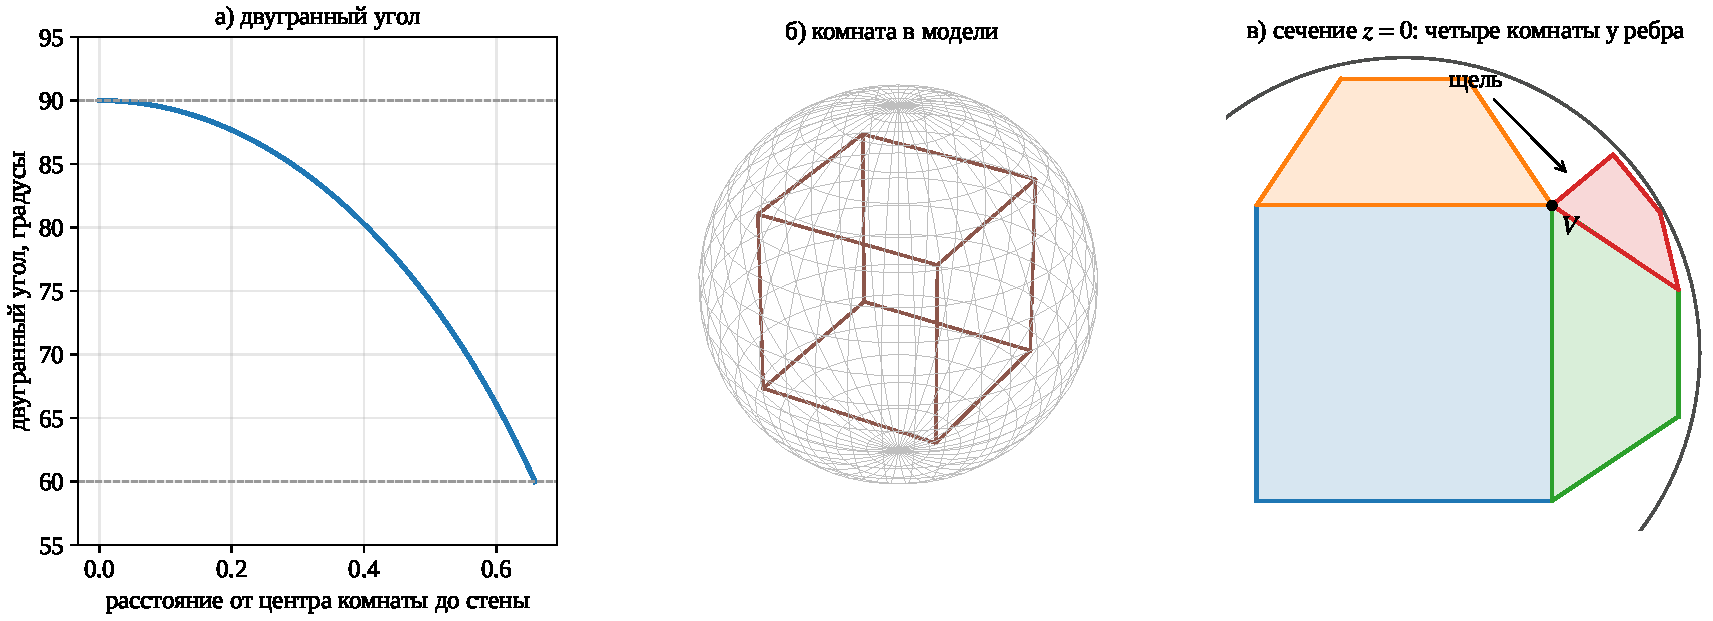
\includegraphics[width=\textwidth]{fig/kub.pdf}
\caption{Кубическая комната: а) двугранный угол в зависимости от расстояния от центра до стены; б) комната в модели при $t=0{,}5$; в) сечение плоскостью $z=0$: исходная комната (синяя) и три её отражения у вершины $V$; между красной и оранжевой остаётся щель}
\label{fig:kub}
\end{figure}

Теорема~\ref{thm:kub}~--- пространственный вариант отсутствия прямоугольников (п.~3.1): из шести плоских стен нельзя собрать комнату, у которой все углы прямые. Если у правильного многогранника с центром в центре шара грани лежат на расстоянии $h$ (в координатах модели) от центра, а нормали соседних граней образуют евклидов угол $\varphi$, то, повторяя доказательство, получаем
\begin{equation}\label{eq:mnogogrannik}
\cos\alpha=\frac{h^2-\cos\varphi}{1-h^2}.
\end{equation}

\subsection{Комнаты-додекаэдры}

Для правильного додекаэдра $\cos\varphi=1/\sqrt5$. По формуле~\eqref{eq:mnogogrannik} угол $\alpha$ становится прямым при $h^2=1/\sqrt5$, то есть $h=5^{-1/4}\approx0{,}6687$. Вершины такого додекаэдра в модели лежат на расстоянии $t\approx0{,}8415$ от центра шара, расстояние от центра до грани равно $\operatorname{arth}h\approx0{,}808$, до вершины~--- $\operatorname{arth}t\approx1{,}226$.

Двугранный угол $\pi/2$ означает, что вокруг каждого ребра сходятся ровно четыре таких додекаэдра. Отражая додекаэдр в его гранях, получают заполнение всего пространства Лобачевского прямоугольными додекаэдрами без щелей и наложений~[11]. Получается дом из одинаковых комнат с прямыми углами, только у каждой комнаты двенадцать стен, и каждая стена~--- правильный пятиугольник.

\subsection{Комната с полом-орисферой}

Есть и другой способ получить комнату с прямыми углами: отказаться от плоского пола. Пусть $\ell=(1,0,0,1)$; это точка $\omega=(0,0,1)$ абсолюта. Возьмём
\begin{itemize}
  \item пол~--- орисферу $\sk{X}{\ell}=-1$ с координатами $u=(u_1,u_2)$ из доказательства теоремы~\ref{thm:krivizna};
  \item потолок~--- концентрическую орисферу $\sk{X}{\ell}=-e^{-h}$;
  \item четыре стены~--- плоскости с полюсами
  \[
  P_{\pm1}=(\pm a,\,1,\,0,\,\pm a),\qquad P_{\pm2}=(\pm a,\,0,\,1,\,\pm a).
  \]
\end{itemize}

\begin{theorem}\label{thm:komnata}
У такой комнаты все двугранные углы между стенами, а также между стенами и полом или потолком прямые; противоположные стены параллельны. Пол~--- евклидов квадрат со стороной $2a$, который можно замостить евклидовыми квадратами, потолок~--- евклидов квадрат со стороной $2ae^{-h}$, высота комнаты равна $h$.
\end{theorem}
\begin{proof}
Все полюсы нормированы: $\sk{P_{\pm1}}{P_{\pm1}}=-a^2+1+a^2=1$. Каждый из них удовлетворяет условию $\sk{P}{\ell}=0$, поэтому точка $\ell$ лежит на каждой стене, и стены состоят из прямых связки параллельных прямых $B_\ell$. По теореме~\ref{thm:svyazka} эти прямые перпендикулярны полу и потолку, значит, перпендикулярны им и стены.

Точка пола $X(u)$ лежит на стене с полюсом $P_{\pm1}$ тогда и только тогда, когда
\[
\sk{X(u)}{P_{\pm1}}=\mp a+u_1=0,
\]
так как слагаемое с $|u|^2$ уничтожается благодаря $\sk{\ell}{P_{\pm1}}=0$. Значит, стены высекают на полу прямые $u_1=\pm a$, $u_2=\pm a$, и по теореме~\ref{thm:krivizna} пол~--- евклидов квадрат со стороной $2a$. Соседние стены перпендикулярны, так как $\sk{P_1}{P_2}=-a^2+a^2=0$; противоположные стены параллельны, так как $\sk{P_1}{P_{-1}}=a^2+1-a^2=1$ (п.~5.3). Наконец, по замечанию в конце п.~5.7 потолок лежит на расстоянии $h$ от пола по прямым связки, и длины на нём в $e^{h}$ раз меньше.
\end{proof}

Комната, все углы которой прямые, в пространстве Лобачевского существует, но за это приходится платить: пол и потолок у неё изогнуты, потому что это орисферы, и потолок меньше пола. Потолок вдвое меньше пола при высоте $h=\ln2\approx0{,}693$. Стены сходятся к точке $\omega$ на абсолюте, и в модели комната похожа на усечённую пирамиду с выпуклыми основаниями (рисунок~\ref{fig:komnata}).

\begin{figure}[H]
\centering
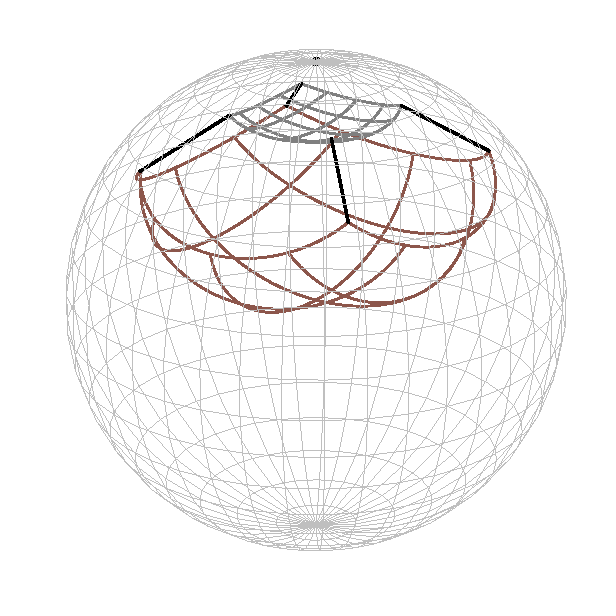
\includegraphics[width=0.6\textwidth]{fig/komnata.pdf}
\caption{Комната с полом-орисферой в модели: пол (коричневая сетка из евклидовых квадратов), потолок (серая сетка), четыре вертикальных ребра~--- прямые связки, сходящиеся в точке $\omega$ абсолюта; $a=1{,}2$, $h=0{,}9$}
\label{fig:komnata}
\end{figure}

\subsection{Интерактивная модель «Круг Кэли~--- Клейна»}

По формулам работы создана веб-страница «Круг Кэли~--- Клейна» (приложение~А). Она состоит из двадцати одной сцены: четырнадцать относятся к плоскости (разделы~1--4), семь~--- к пространству (разделы~5 и~6), и каждая посвящена одному утверждению или одной группе утверждений (таблица~\ref{tab:sceny}). В сценах на плоскости точки и концы хорд передвигаются мышью или пальцем, в сценах в пространстве рисунок можно поворачивать, а параметры задаются ползунками. Рядом с рисунком приведены формулировка утверждения, вычисленные величины и вопросы к сцене.

\begin{table}[H]
\caption{Сцены интерактивной модели}
\label{tab:sceny}
\centering
\singlespacing\footnotesize
\begin{tabular}{|c|>{\raggedright\arraybackslash}p{5.4cm}|>{\raggedright\arraybackslash}p{6.6cm}|c|}
\hline
№ & Сцена & Что показывает & Пункт \\ \hline
1 & Модель Кэли~--- Клейна & длина через сложное отношение, деления равной длины & 1.3 \\ \hline
2 & π-движения & сохранение длин и углов при переносе фигуры & 1.3 \\ \hline
3 & Аксиома Лобачевского & пучок прямых через точку, две параллельные & 2.1 \\ \hline
4 & Параллельность через внутренний луч & точка пересечения внутреннего луча с прямой уходит на абсолют & 2.1 \\ \hline
5 & Биссектраль и равнонаклонные & ось симметрии двух параллельных & 2.1 \\ \hline
6 & Функция Лобачевского & угол параллельности и его график & 2.2 \\ \hline
7 & Общий перпендикуляр и расстояние & построение через полюсы, график расстояния & 2.3, 2.4 \\ \hline
8 & Сумма углов и средняя линия & сумма углов, дефект, дополнительные построения & 3.1 \\ \hline
9 & Серединные перпендикуляры & треугольник и серединные перпендикуляры к его сторонам & 3.5 \\ \hline
10 & Двупрямоугольник и четырёхугольник Саккери & углы и стороны при изменении длин & 3.2 \\ \hline
11 & Окружность, эквидистанта, орицикл & оси, касательные, хорды & 3.3, 5.2 \\ \hline
12 & Острый угол и заградительная прямая & перпендикуляры к стороне угла, граничная точка & 3.4 \\ \hline
13 & Независимость аксиомы параллельности & евклидова плоскость и модель рядом & 4.2 \\ \hline
14 & Евклид и Лобачевский & сводный перечень утверждений со ссылками на сцены & --- \\ \hline
15 & Сфера & эллипсоид, изображение центра и евклидов центр, кривизна & 5.6, 5.7 \\ \hline
16 & От сферы к орисфере & сферы через одну точку с центром, уходящим к абсолюту & 5.5 \\ \hline
17 & Орисфера и её сетка & связка параллельных прямых, евклидова сетка на орисфере & 5.7 \\ \hline
18 & Эквидистантная поверхность & перпендикуляры к плоскости через её полюс & 5.6 \\ \hline
19 & Кубическая комната & двугранный угол и щель между четырьмя комнатами у ребра & 6.2 \\ \hline
20 & Комната-додекаэдр & прямой двугранный угол, четыре комнаты у ребра & 6.3 \\ \hline
21 & Комната с полом-орисферой & пол, потолок и стены, отношение сторон & 6.4 \\ \hline
\end{tabular}
\end{table}

Все величины на панели вычисляются по формулам разделов~1 и~5. Перпендикуляр строится через полюс (лемма~\ref{lem:polyus}), углы находятся по предложению~\ref{prop:ugol} или после переноса вершины в центр сдвигом~\eqref{eq:sdvig}, длины~--- по предложению~\ref{prop:ch}, симметрии~--- по формуле~\eqref{eq:otrazhenie}, окружности, эквидистанты и орициклы~--- по уравнениям~\eqref{eq:klein-traektoriya}. Перед публикацией вычислительное ядро проверено на 2000 случайных наборах точек. Длина через сложное отношение совпала с формулой~\eqref{eq:ch}, движения сохраняли длины и углы, угол между перпендикуляром, построенным через полюс, и прямой оказался прямым, точки построенных окружностей, эквидистант и орициклов лежали на нужном расстоянии; наибольшее отклонение во всех проверках не превысило $10^{-12}$. Страница написана на языке JavaScript и состоит из одного файла, поэтому её можно открыть в любом браузере, в том числе на телефоне.

Углы на рисунке модели искажены, и это одна из причин держать числа рядом с рисунком: трапеция на рисунке~\ref{fig:sakkeri} выглядит как евклидова, а её верхние углы равны $54{,}3^\circ$.

\subsection{Модели поверхностей на языке Python}

Модели гиперболической сферы и орисферы написаны также на языке Python с библиотеками Plotly и Dash (приложение~А). В модели сферы задаются гиперболический центр и гиперболический радиус $\rho$, а эллипсоид строится по формулам~\eqref{eq:sfera-poluosi}; хорды, проходящие через центр, пересекают его в точках, вычисленных по тем же формулам. Проверка на 48 наборах параметров показала, что все точки поверхности и все 2400 точек входа и выхода хорд удалены от центра на $\rho$ с точностью порядка $10^{-12}$. Модель орисферы использует параметр $k'$, связанный с полуосью формулой $r^2=k'/(1+k')$; в обозначениях п.~5.6 это $k'=c^2$.

Следующий шаг работы~--- модель комнаты, которую можно рассматривать изнутри. Её удобно строить тоже в модели Кэли~--- Клейна. Если наблюдатель находится в центре шара, направления на точки пространства изображаются без искажений, а перемещение наблюдателя заменяется π-движением всего пространства, то есть умножением однородных координат на матрицу, сохраняющую форму абсолюта. Видеокарта сама выполняет переход от однородных координат к точке шара, плоские грани остаются плоскими, и изображение получается точным; разбивать на мелкие части нужно только кривые поверхности, например пол-орисферу.

\section{Задачи}

Задачи~7.1--7.4 решаются средствами абсолютной геометрии и геометрии Лобачевского, задачи~7.5--7.11~--- с помощью модели. В задачах~7.2 и~7.4 приведено по два решения: синтетическое и в модели.

\begin{task}
Выпуклый $n$-угольник $F$ разбит диагоналями, выходящими из одной вершины, на $n-2$ треугольника. Докажите, что сумма дефектов этих треугольников равна $(n-2)\pi-s(F)$, где $s(F)$~--- сумма углов многоугольника. Выведите отсюда, что эта сумма не зависит от выбора вершины.
\end{task}
\textit{Решение.} Каждый угол многоугольника либо совпадает с углом одного из треугольников, либо (в вершине, из которой проведены диагонали) складывается из углов нескольких треугольников. Других углов у треугольников нет: все их вершины~--- вершины многоугольника. Поэтому сумма углов всех треугольников равна $s(F)$, и
\[
\sum_{i=1}^{n-2}\bigl(\pi-s_i\bigr)=(n-2)\pi-\sum_{i=1}^{n-2}s_i=(n-2)\pi-s(F).
\]
Правая часть от выбора вершины не зависит. Это позволяет назвать число $\delta(F)=(n-2)\pi-s(F)$ дефектом многоугольника.

\begin{task}
На плоскости даны пучок прямых $P$ и прямая $l$, не принадлежащая пучку. Существует ли прямая пучка, перпендикулярная $l$, и сколько их, если $P$~--- пучок а)~пересекающихся, б)~параллельных, в)~расходящихся прямых?
\end{task}
\textit{Решение 1.} а) Из центра пучка на прямую $l$ можно опустить единственный перпендикуляр, он принадлежит пучку. б) Пусть $\Omega$~--- общая точка абсолюта прямых пучка; она не является концом $l$, иначе $l$ принадлежала бы пучку. Через $\Omega$ проходит единственная прямая, перпендикулярная $l$~[1]. в) Прямая пучка перпендикулярна базе $a$; если она перпендикулярна и $l$, то это общий перпендикуляр $a$ и $l$. По теореме~\ref{thm:perpendikulyar} он существует и единствен, если $a$ и $l$ расходятся, и не существует, если они пересекаются или параллельны.

\textit{Решение 2.} Пусть пучок задан точкой $V$ (предложение~\ref{prop:puchok}), а $P_l$~--- полюс прямой $l$. По лемме~\ref{lem:polyus} прямая перпендикулярна $l$ тогда и только тогда, когда её продолжение проходит через $P_l$. Значит, искомая прямая~--- это евклидова прямая $VP_l$ (точки различны, так как $l$ не принадлежит пучку), и ответ зависит только от того, пересекает ли она круг. В случае а) $V$ лежит внутри круга, и пересечение есть. В случае б) $V$ лежит на абсолюте и не является концом хорды $l$; прямая $VP_l$ не касается абсолюта в точке $V$, так как касательная в $V$ есть поляра $V$, а $P_l$ на ней не лежит (иначе $V$ лежала бы на поляре $P_l$, то есть была бы концом $l$). Значит, прямая $VP_l$ пересекает круг. В случае в) $V$~--- полюс базы $a$, прямая $VP_l$ есть прямая через полюсы $a$ и $l$, и по теореме~\ref{thm:perpendikulyar} она пересекает круг ровно тогда, когда $a$ и $l$ расходятся.

\textit{Ответ:} в случаях а) и б) такая прямая единственна, в случае в) она существует (и единственна) тогда и только тогда, когда база пучка и прямая $l$ расходятся.

\begin{task}
Найдите дефект пятиугольника $ABCDE$, если $ABCD$~--- выпуклый четырёхугольник с углами $\angle A=\angle B=\angle C=90^\circ$, $\angle D=60^\circ$, а $ADE$~--- равносторонний треугольник с углами $\alpha$, построенный во внешнюю сторону от четырёхугольника.
\end{task}
\textit{Решение.} Треугольник $ADE$ построен во внешнюю сторону от четырёхугольника, то есть лежит по другую сторону от прямой $AD$. Поэтому в вершинах $A$ и $D$ углы четырёхугольника и треугольника прилегают друг к другу по общей стороне $AD$ и складываются. Углы пятиугольника: $\angle A=\pi/2+\alpha$, $\angle B=\angle C=\pi/2$, $\angle D=\pi/3+\alpha$, $\angle E=\alpha$. Их сумма равна $11\pi/6+3\alpha$, и
\[
\delta(ABCDE)=3\pi-\Bigl(\frac{11\pi}6+3\alpha\Bigr)=\frac{7\pi}6-3\alpha.
\]
Проверка: дефект аддитивен, $\delta(ABCD)=2\pi-11\pi/6=\pi/6$, $\delta(ADE)=\pi-3\alpha$, и сумма даёт тот же ответ.

\textit{Ответ:} $\dfrac{7\pi}{6}-3\alpha$.

\begin{task}
В выпуклом четырёхугольнике $ABCD$ углы $A$ и $B$ равны. Докажите, что серединный перпендикуляр $m$ к стороне $AB$ принадлежит пучку, которому принадлежат прямые $AD$ и $BC$.
\end{task}
\textit{Решение 1.} Симметрия $\sigma$ относительно $m$ меняет местами точки $A$ и $B$. Так как $\angle DAB=\angle CBA$ и точки $C$, $D$ лежат по одну сторону от $AB$, симметрия переводит луч $AD$ в луч $BC$, а значит, меняет местами прямые $AD$ и $BC$.

Если прямые $AD$ и $BC$ пересекаются в точке $O$, то $\sigma(O)$ лежит на обеих прямых, то есть $\sigma(O)=O$, и $O\in m$. Если они параллельны, то их общая точка абсолюта переходит в себя, поэтому она является концом прямой $m$, и $m$ параллельна обеим прямым в том же направлении. Если они расходятся, то их общий перпендикуляр $PQ$ ($P\in AD$, $Q\in BC$) переходит в общий перпендикуляр тех же прямых, то есть в себя, причём $\sigma(P)=Q\ne P$. Прямая, переходящая в себя при симметрии, либо совпадает с осью симметрии, либо ей перпендикулярна. Совпасть с $m$ прямая $PQ$ не может (точки $m$ неподвижны), поэтому $PQ\perp m$, и $m$ принадлежит пучку с базой $PQ$.

\textit{Решение 2.} Пусть $V$~--- точка пересечения евклидовых прямых, содержащих хорды $AD$ и $BC$; по предложению~\ref{prop:puchok} она задаёт пучок. Симметрия $\sigma$~--- проективное преобразование, которое меняет местами эти две прямые, поэтому их точку пересечения оставляет на месте: $\sigma(V)=V$. По формуле~\eqref{eq:otrazhenie} неподвижные точки $\sigma$~--- точки прямой $m$ и её полюс $P_m$. Если $V=P_m$, то по лемме~\ref{lem:polyus} прямые $AD$ и $BC$ перпендикулярны $m$; но прямая, перпендикулярная оси, переходит при симметрии в себя, а $\sigma$ переводит $AD$ в $BC\ne AD$. Значит, $V$ лежит на прямой, содержащей хорду $m$, и $m$ принадлежит пучку $B_V$. Это одно рассуждение для всех трёх случаев.

\begin{task}
Найдите угол параллельности отрезка, который изображается в модели отрезком от центра круга до точки $(0{,}6;\,0)$.
\end{task}
\textit{Решение.} По следствию~\ref{cor:ot-centra} длина отрезка равна $x=\operatorname{arth}0{,}6=\tfrac12\ln\tfrac{1{,}6}{0{,}4}=\ln2$. По теореме~\ref{thm:lobachevsky} $\cos\Pi(x)=\thh x=0{,}6$, откуда $\Pi(x)\approx53{,}13^\circ$. Проверка по второй формуле: $\operatorname{tg}\frac{\Pi}{2}=e^{-\ln2}=\frac12$, и $2\operatorname{arctg}\frac12\approx53{,}13^\circ$.

\textit{Ответ:} $\Pi(\ln 2)=\arccos0{,}6\approx53{,}13^\circ$.

\begin{task}
Прямые изображены хордами $k_2=0{,}3$ и $k_2=-0{,}5$. Определите их взаимное расположение и найдите длину общего перпендикуляра, если он есть.
\end{task}
\textit{Решение.} Содержащие хорды евклидовы прямые параллельны, их общая точка бесконечно удалена и лежит вне круга, поэтому прямые расходятся. Обе хорды евклидово перпендикулярны вертикальному диаметру, и по лемме~\ref{lem:polyus} он перпендикулярен обеим прямым; это и есть общий перпендикуляр (теорема~\ref{thm:perpendikulyar}). Центр лежит между его концами $(0;\,0{,}3)$ и $(0;\,-0{,}5)$, поэтому по следствию~\ref{cor:ot-centra} длина равна $\operatorname{arth}0{,}3+\operatorname{arth}0{,}5\approx0{,}3095+0{,}5493=0{,}8588$.

\textit{Ответ:} прямые расходятся, длина общего перпендикуляра $\approx0{,}859$.

\begin{task}
Найдите углы и сумму углов четырёхугольника Саккери, у которого основание и боковые стороны равны $1$.
\end{task}
\textit{Решение.} По формуле~\eqref{eq:sakkeri} при $b=h=1$
\[
\cos\gamma=\frac{\sh0{,}5\cdot\sh1}{\sqrt{\ch^20{,}5+\sh^20{,}5\cdot\sh^21}}\approx\frac{0{,}5211\cdot1{,}1752}{\sqrt{1{,}2715+0{,}2715\cdot1{,}3811}}\approx0{,}4772,
\]
$\gamma\approx61{,}49^\circ$. Сумма углов равна $2\cdot90^\circ+2\gamma\approx302{,}99^\circ$, дефект $\approx57{,}01^\circ$.

\textit{Ответ:} $\angle C=\angle D\approx61{,}49^\circ$, сумма углов $\approx302{,}99^\circ$.

\begin{task}
Найдите в модели уравнение орицикла, который касается абсолюта в точке $(1,0)$ и проходит через центр круга. Найдите центр и полуоси эллипса, которым он изображается.
\end{task}
\textit{Решение.} По формуле~\eqref{eq:klein-traektoriya} с $\omega=(1,0)$ уравнение имеет вид $(1-x)^2=c^2(1-x^2-y^2)$. Подстановка $x=y=0$ даёт $c=1$, и
\[
(1-x)^2=1-x^2-y^2\iff 2x^2-2x+y^2=0\iff\frac{(x-1/2)^2}{1/4}+\frac{y^2}{1/2}=1.
\]
\textit{Ответ:} эллипс с центром $(1/2,\,0)$, полуосью $1/2$ вдоль оси $Ox$ и полуосью $1/\sqrt2$ поперёк неё. Это согласуется с п.~5.6: $r=c/\sqrt{1+c^2}=1/\sqrt2$, $r^2=1/2$, центр $(1-r^2)\omega$.

\begin{task}
При каком расстоянии от центра кубической комнаты до стены её двугранный угол равен $80^\circ$?
\end{task}
\textit{Решение.} Из формулы~\eqref{eq:kub} $t^2=\cos80^\circ/(1+\cos80^\circ)\approx0{,}1480$, $t\approx0{,}3847$, $d=\operatorname{arth}t\approx0{,}406$.

\textit{Ответ:} примерно $0{,}406$ радиуса кривизны.

\begin{task}
Комната с полом-орисферой (п.~6.4) имеет высоту $h$. При какой высоте потолок вдвое меньше пола по длине стороны? Во сколько раз он меньше при $h=1$?
\end{task}
\textit{Решение.} По теореме~\ref{thm:komnata} сторона потолка равна стороне пола, умноженной на $e^{-h}$. Условие $e^{-h}=1/2$ даёт $h=\ln2\approx0{,}693$; при $h=1$ потолок меньше в $e\approx2{,}718$ раза.

\begin{task}
Докажите, что евклидов центр эллипсоида, изображающего сферу в модели, лежит на отрезке между центром шара и изображением центра сферы и совпадает с последним только при $q=0$.
\end{task}
\textit{Решение.} По п.~5.6 евклидов центр равен $q/B$, где $B=a^2+C(1-a^2)$, $C=\ch^2\rho$. Тогда $B-1=(C-1)(1-a^2)>0$ при $\rho>0$ и $a<1$, поэтому $0<1/B<1$, и точка $q/B$ лежит на отрезке между $0$ и $q$, не совпадая с $q$ при $q\ne0$.

\structsection{ЗАКЛЮЧЕНИЕ}

В работе построены интерпретации основных утверждений планиметрии Лобачевского в модели Кэли~--- Клейна. Модель описана на языке абсолюта: полюс и поляра, сложное отношение, π-движения как проективные преобразования, сохраняющие форму абсолюта. Симметрия относительно прямой записана формулой~\eqref{eq:otrazhenie}, и из неё выведено правило, на котором держатся почти все построения: перпендикуляр к хорде проходит через её полюс.

С помощью этого правила в модели получены явные формулы. Если поместить вершину угла параллельности в центр круга, формула Лобачевского $\operatorname{tg}\frac{\Pi(x)}2=e^{-x}$ получается в две строки. Расстояние от точки до диаметра~\eqref{eq:do-diametra} даёт явный вид теорем о расстоянии между точками параллельных и расходящихся прямых и уравнение эквидистанты. Общий перпендикуляр расходящихся прямых~--- хорда через их полюсы, и признак расходящихся прямых сводится к тому, лежит ли точка пересечения продолжений хорд вне круга. Для четырёхугольника Саккери найдена формула угла при верхнем основании~\eqref{eq:sakkeri}. В отрицании предложения Лежандра граничная точка оказалась связана с углом параллельности: $\Pi(OP^*)$ равен данному углу.

В разделах~5 и~6 те же средства применены к пучкам и связкам прямых. Траектория пучка и поверхность, ортогональная связке, задаются одним условием $\sk{X}{V}=c$, а три типа (окружность, орицикл, эквидистанта и соответствующие поверхности) различаются только положением точки $V$: внутри круга, на абсолюте или вне его. Найдены точные изображения сферы, орисферы и эквидистантной поверхности и их внутренняя кривизна. Показано, что кубическая комната в пространстве Лобачевского не может иметь прямых углов, а комната с полом и потолком из концентрических орисфер может, причём её потолок в $e^{h}$ раз меньше пола.

По формулам работы создана веб-страница «Круг Кэли~--- Клейна» из двадцати одной сцены. В четырнадцати сценах на плоскости фигуры модели можно передвигать и сразу видеть вычисленные длины и углы, в семи сценах в пространстве показаны сфера, орисфера, эквидистантная поверхность и три комнаты. Следующие шаги~--- объединить все модели на одном сайте и построить модель комнаты, которую можно рассматривать изнутри.

\structsection{СПИСОК ИСПОЛЬЗОВАННЫХ ИСТОЧНИКОВ}

\begin{enumerate}[label=\arabic*.,leftmargin=*,labelindent=\parindent,itemsep=0pt]
  \item Атанасян, Л.\,С. Геометрия Лобачевского / Л.\,С.~Атанасян.~--- Москва\,: БИНОМ. Лаборатория знаний, 2014.~--- 320\,с.
  \item Атанасян, Л.\,С. Геометрия. Ч.\,2 / Л.\,С.~Атанасян, В.\,Т.~Базылев.~--- Москва\,: Просвещение, 1987.~--- 368\,с.
  \item Ефимов, Н.\,В. Высшая геометрия / Н.\,В.~Ефимов.~--- Москва\,: Наука, 1971.~--- 584\,с.
  \item Каган, В.\,Ф. Основания геометрии. Ч.\,2 / В.\,Ф.~Каган.~--- Москва\,; Ленинград\,: ГИТТЛ, 1949.~--- 340\,с.
  \item Норден, А.\,П. Элементарное введение в геометрию Лобачевского / А.\,П.~Норден.~--- Москва\,: ГИТТЛ, 1953.~--- 216\,с.
  \item Прасолов, В.\,В. Геометрия Лобачевского / В.\,В.~Прасолов.~--- Москва\,: МЦНМО, 2004.~--- 208\,с.
  \item Шафаревич, И.\,Р. Линейная алгебра и геометрия / И.\,Р.~Шафаревич, А.\,О.~Ремизов.~--- Москва\,: Физматлит, 2009.~--- 512\,с.
  \item Широков, П.\,А. Краткий очерк основ геометрии Лобачевского / П.\,А.~Широков.~--- Москва\,: Наука, 1983.~--- 208\,с.
  \item Ratcliffe, J.\,G. Foundations of Hyperbolic Manifolds / J.\,G.~Ratcliffe.~--- 3rd ed.~--- Cham\,: Springer, 2019.~--- (Graduate Texts in Mathematics\,; vol.~149). \todo{сверить выходные данные, число страниц}
  \item Cannon, J.\,W. Hyperbolic geometry / J.\,W.~Cannon, W.\,J.~Floyd, R.~Kenyon, W.\,R.~Parry // Flavors of Geometry / ed. by S.~Levy.~--- Cambridge\,: Cambridge University Press, 1997.~--- (MSRI Publications\,; vol.~31).~--- P.~59--115. \todo{сверить}
  \item Coxeter, H.\,S.\,M. Regular honeycombs in hyperbolic space / H.\,S.\,M.~Coxeter // Proceedings of the International Congress of Mathematicians, 1954.~--- Amsterdam, 1956.~--- Vol.~III.~--- P.~155--169. \todo{сверить}
\end{enumerate}

\structsection{ПРИЛОЖЕНИЕ А}
\begin{center}
(справочное)\\
\textbf{Компьютерные модели и численная проверка формул}
\end{center}

Интерактивная модель «Круг Кэли~--- Клейна» (плоскость и пространство): \todo{адрес страницы после публикации на сайте}.

Модели на языке Python опубликованы в репозиториях:
\begin{itemize}
  \item гиперболическая сфера: \url{https://github.com/mvbulgakova/hyperbolic-geometry-app};
  \item орисфера: \url{https://github.com/mvbulgakova/hyperbolic-geometry2-app}.
\end{itemize}

Формулы п.~5.6 проверялись программой, приведённой ниже. Для точек построенной сферы вычисляется расстояние до центра по предложению~\ref{prop:ch}, для точек орисферы~--- величина $(1-k\cdot\omega)/\sqrt{1-|k|^2}$, которая должна быть постоянной. На 200 случайных наборах параметров (центр на расстоянии до $0{,}95$ от центра шара, $0{,}05\le\rho\le2{,}5$, $0{,}05\le r\le0{,}95$) наибольшее отклонение составило $4\cdot10^{-13}$ для сферы и $4\cdot10^{-10}$ для орисферы; для центров на расстоянии $0{,}99$ относительная ошибка не превысила $6\cdot10^{-11}$.

{\singlespacing\small
\begin{Verbatim}
import numpy as np
from klein_surfaces import hyperbolic_sphere, horosphere

rng = np.random.default_rng(1)

def points(mesh, eps):
    k = np.stack([m.ravel() for m in mesh], 1)
    return k[1 - (k * k).sum(1) > eps]

def unit(v):
    return v / np.linalg.norm(v)

def distance(k, c):
    return np.arccosh((1 - k @ c) /
                      np.sqrt((1 - (k * k).sum(1)) * (1 - c @ c)))

def horo_const(k, omega):
    return (1 - k @ omega) / np.sqrt(1 - (k * k).sum(1))

worst_sphere = 0
for _ in range(200):
    c = unit(rng.normal(size=3)) * rng.uniform(0, 0.95)
    rho = rng.uniform(0.05, 2.5)
    k = points(hyperbolic_sphere(c, rho), 1e-12)
    worst_sphere = max(worst_sphere, np.abs(distance(k, c) - rho).max())

worst_horo = 0
for _ in range(200):
    omega = unit(rng.normal(size=3))
    r = rng.uniform(0.05, 0.95)
    k = points(horosphere(omega, r), 1e-6)
    expected = r / np.sqrt(1 - r * r)
    worst_horo = max(worst_horo,
                     np.abs(horo_const(k, omega) - expected).max())
print(worst_sphere, worst_horo)
\end{Verbatim}
}


\end{document}
